%%%%%%%%%%%%%%%%%%%%%%%%%%%%%%%%%%%%%%%%%
% Fancyslides Presentation
% LaTeX Template
% Version 1.0 (30/6/13)
%
% This template has been downloaded from:
% http://www.LaTeXTemplates.com
%
% The Fancyslides class was created by:
% Paweł Łupkowski (pawel.lupkowski@gmail.com)
%
% License:
% CC BY-NC-SA 3.0 (http://creativecommons.org/licenses/by-nc-sa/3.0/)
%
%%%%%%%%%%%%%%%%%%%%%%%%%%%%%%%%%%%%%%%%%

%----------------------------------------------------------------------------------------
%	PACKAGES AND OTHER DOCUMENT CONFIGURATIONS
%----------------------------------------------------------------------------------------

\documentclass{fancyslides}

\usepackage[utf8]{inputenc} % Allows the usage of non-english characters
\usepackage{times} % Use the Times font
\usepackage{booktabs} % Allows the use of \toprule, \midrule and \bottomrule in tables
\graphicspath{{images/}} % Location of the slide background and figure files

% Beamer options - do not change
\usetheme{default} 
\setbeamertemplate{navigation symbols}{} % Disable the slide navigation buttons on the bottom of each slide
\setbeamercolor{structure}{fg=\yourowntexcol} % Define the color of titles and fixed text elements (e.g. bullet points)
\setbeamercolor{normal text}{fg=\yourowntexcol} % Define the color of text in the presentation

%------------------------------------------------
% COLORS
% The following colors are predefined in this class: white, black, gray, blue, green and orange

% Define your own color as follows:
\definecolor{bulgarianrose}{rgb}{0.28,0.02,0.03}
%\definecolor{rose}{rgb}{0.54,0.2,0.14}
%\definecolor{charcoal}{rgb}{0.21,0.27,0.31}
\newcommand{\structureopacity}{0.75} % Opacity (transparency) for the structure elements (boxes and circles)

\newcommand{\strcolor}{bulgarianrose} % Set the color of structure elements (boxes and circles)
\newcommand{\yourowntexcol}{white} % Set the text color

%----------------------------------------------------------------------------------------
%	TITLE SLIDE
%----------------------------------------------------------------------------------------

\newcommand{\titlephrase}{Spatially Random Processes in
  One-Dimensional Maps: The Logistic Map and The Arnold Circle Map} % Presentation title
\newcommand{\name}{Amy Le} % Presenter's name
\newcommand{\affil}{CU Boulder} % Presenter's institution
\newcommand{\email}{April 2, 2015} % Presenter's email address

\begin{document}

\startingslide % This command inserts the title slide as the first slide

%----------------------------------------------------------------------------------------
%	PRESENTATION SLIDES
%----------------------------------------------------------------------------------------

%\fbckg{1.jpg} % Slide background image
\begin{frame}
\itemized{
\item Groundwater Contamination
\item Spatially Random Processes
\item Implementation in the Logistic Map and the Circle Map
}
%\pointedsl{} % Text in this environment is printed in a circle and will be made large and uppercase - if you need to fit more text in you can reduce the font size within the \pointedsl{} bracket as usual, e.g. \pointedsl{\large smaller main point}
\end{frame}
%------------------------------------------------

\begin{frame}
\misc{ % Anything can be placed inside the \misc{} command
The total groundwater withdrawls in the United States in 2005, categorized
  in terms of use.
\begin{figure}[h]
\centering
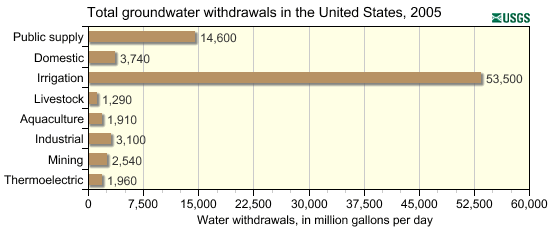
\includegraphics[scale=0.7]{gwuse}
\end{figure}
}
\end{frame}

%------------------------------------------------

\begin{frame}
\misc{ % Anything can be placed inside the \misc{} command
Typical porosity and hydraulic conductivity ranges for clay, sand, and gravel.
\begin {table}[h]
\begin{center}
    \begin{tabular}{ l l l l}
    \toprule
    Grain Size & Material & Porosity & Hydraulic Conductivity $K$
    (m/s)\\ 
\midrule
    Fine & Clay  &  50\% &$[5\times 10^{-9}, 5\times 10^{-6}]$\\ 
    Medium &  Sand & 25\% & $[10^{-8},10^{-6}]$\\ 
    Coarse &  Gravel &  20\% & $[5 \times 10^{-4}, 5 \times 10^{-2}]$\\ 
    \end{tabular}
\end{center}
\end{table}
}
\end{frame}
%------------------------------------------------
\begin{frame}
\misc{ 
\begin{figure}[h]
\centering
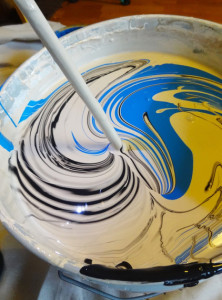
\includegraphics[scale=0.65]{Mixing-Paint-222x300}
\end{figure}
}
\end{frame}

%------------------------------------------------
\begin{frame}
\pointedsl{\large Spatially Random Processes} % Text in this environment is printed in a circle and will be made large and uppercase - if you need to fit more text in you can reduce the font size within the \pointedsl{} bracket as usual, e.g. \pointedsl{\large smaller main point}
\end{frame}
%------------------------------------------------

\begin{frame}
\misc{
Log-normal noise in a homogeneous process
\begin{align*}
\begin{split}
\xi(x)&=\ln(R(x)) \\
\mu &= E[\xi(x)] = \ln(r)\>, \quad  r \in [0,\infty)\\
C(\xi(y+x),\xi(y)) &= E[(\xi(y+x) - E[\xi(y+x)])(\xi(y) -E[\xi(y)])]\\
&= E[(\xi(y+x) -\ln(r))(\xi(y)-\ln(r))]
%\sigma^2 &= E[(\xi(x) - \mu)^2]=E[\xi(x)^2]-(\ln(r))^2.
\end{split}
\end{align*}
}
\end{frame}
%------------------------------------------------
\begin{frame}
%\framedsl{} 
\misc{Normal noise
\begin{align*}
\begin{split}
\xi(x)&= \ln(r) + \sum_{n \in \mathbb{Z}}\hat{\xi}_ne^{2\pi inx}\\
\hat{\xi}_{n}^* &= \hat{\xi}_{-n} \>, \quad  \hat{\xi}_n \in \mathbb{C}\\
\hat{\mu}_n&=E[\hat{\xi}_n]=0\\
\hat{\sigma}_n^2&=E[\hat{\xi}_n^2]=E[|\hat{\xi}_n|^2]=S(n)
\end{split}
\end{align*}
}
\end{frame}
%------------------------------------------------
\begin{frame}
\misc{
Spectral density, variance of $\hat{\xi}_n$, and covariance of $\xi(x)$
\begin{align*}
\begin{split}
\hat{\sigma}_n^2&=S(n)\\
S(n)&=\alpha e^{-L|n|}\>, \quad  L \in (0,\infty), \alpha \in \mathbb{R}\\
C(x) &= \sum_{n\in \mathbb{Z}}S(n)e^{2\pi inx}\\
&=\alpha \frac{e^{2L}-1}{e^{2L}-2\cos(2\pi x)e^L+1}\\
\end{split}
\end{align*}
}
\end{frame}
%------------------------------------------------
\begin{frame}
\misc{
Expressing $\alpha$\\
\begin{align*}
\begin{split}
C(0,y) &= E[(\xi(y+x) -\ln(r))(\xi(y)-\ln(r))]=\sigma^2\\
\alpha &= \sigma^2 \tanh(L/2)\\
\end{split}
\end{align*}
}
\end{frame}

%------------------------------------------------
\begin{frame}
\misc{ 
\begin{itemize}
\item The correlation function $C(x)$
\item The spectral density $S(n)$
\end{itemize}
$L=0.5,\sigma=0.0216, \alpha=0.000114$
\begin{figure}[h]
\centering
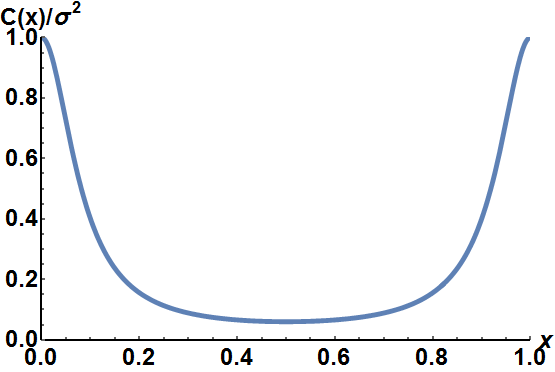
\includegraphics[width=.48\textwidth]{cx}\hfill
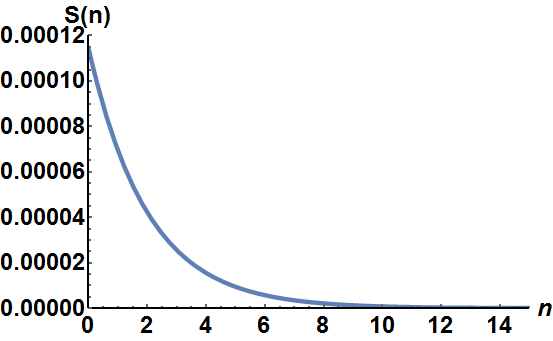
\includegraphics[width=.51\textwidth]{sn}
\end{figure}
}
\end{frame}
%------------------------------------------------
\begin{frame}
\misc{ The correlation function $C(x)$ for $L \in \{0.1,0.5,1\}$. 
\begin{figure}[h]
\centering
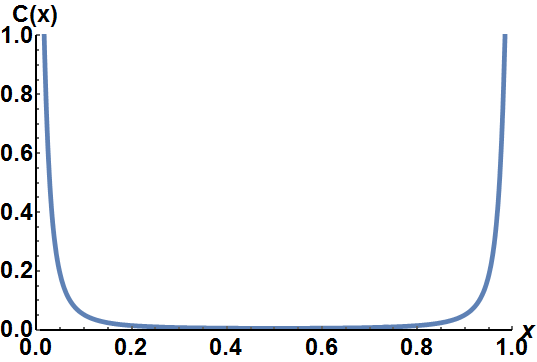
\includegraphics[width=.33\textwidth]{correlation_L01}\hfill
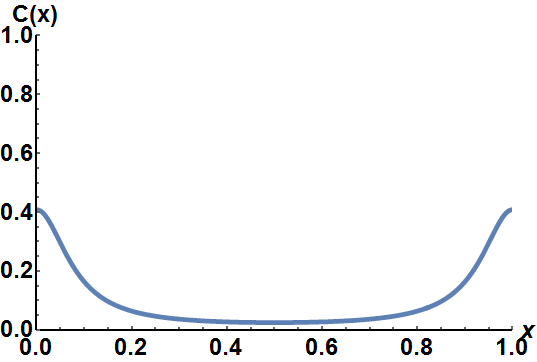
\includegraphics[width=.33\textwidth]{correlation_L05}\hfill
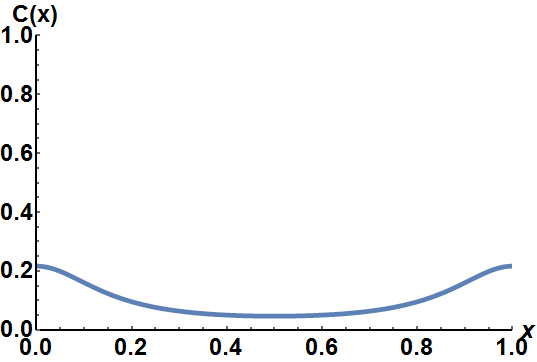
\includegraphics[width=.33\textwidth]{correlation_L1}
\end{figure}
}
\end{frame}
%------------------------------------------------
\begin{frame}
\pointedsl{\small Distributions of Random Variables} 
 \end{frame}

%------------------------------------------------

\begin{frame}
\misc{
Choosing a distribution: uniform 
\begin{align*}
\begin{split}
\hat{\xi}_n &\sim Unif(-M_n,M_n)
\end{split}
\end{align*}
\begin{equation*}
   h_u(a_n,b_n)= \left\{
     \begin{array}{lr}
       \frac{1}{4 M_n^2} & |a_n|,|b_n| \leq M_n\\
       0 & |a_n|,|b_n| > M_n\\
     \end{array}
   \right.
\end{equation*} 
}
\end{frame}
%------------------------------------------------
\begin{frame}
\misc{Expressing $M_n$
\begin{align*}
\begin{split}
S(n) &= E[|\hat{\xi}_n|^2]\\
M_n &= \sqrt{\frac{3}{2}S(n)}\\
\end{split}
\end{align*}
}
\end{frame}
%------------------------------------------------

\begin{frame}
\misc{ % Anything can be placed inside the \misc{} command
The function $R:[0,1]\to [0,4]$ where $\hat{\xi}_n \sim
Unif(-M_n,M_n), \sigma=0.0386, L=0.1, r=3.5, N=100$
\begin{figure}[h]
\centering
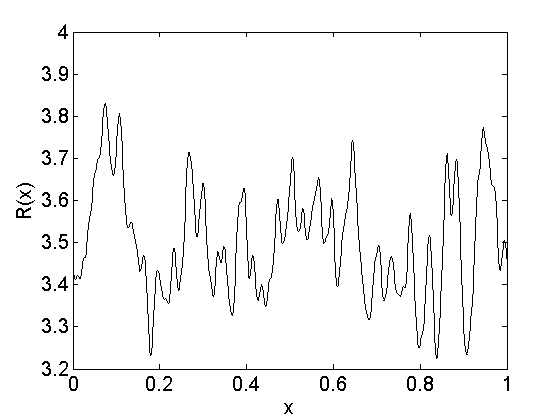
\includegraphics[scale=0.5]{xi}
\end{figure}
}
\end{frame}

%------------------------------------------------
\begin{frame}
\misc{
Choosing a distribution: Gaussian 
\begin{equation*}
\hat{\xi}_n \sim N(0,\hat{\sigma}_n^2)
\end{equation*}
\begin{equation*}
   h_g(x) = \frac{1}{\hat{\sigma}_n \sqrt{2\pi}}e^{-\frac{x^2}{2\hat{\sigma}_n^2}}
\end{equation*} 
}
\end{frame}

%------------------------------------------------

\begin{frame}
\misc{ 
The function $\Omega:\mathbb{R}^+ \to \mathbb{R}^+$ where $\hat{\xi}_n \sim
N(0,\hat{\sigma}_n^2), L=0.1, r=0.7, \alpha = 10^{-6}, N=100$
\begin{figure}[h]
\centering
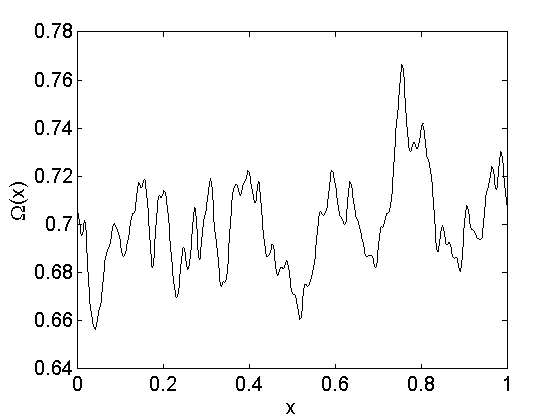
\includegraphics[scale=0.5]{Omega}
\end{figure}
}
\end{frame}
%------------------------------------------------
\begin{frame}
\pointedsl{\large One-Dimensional Maps} 
 \end{frame}

%------------------------------------------------

\fbckg{blank}
\begin{frame}
\framedsl{Logistic Map} 
\misc{
\begin{align*}
\begin{split}
x_{n+1}= f_l(x_n) &=  rx_n(1-x_n)\>, \quad  r \in [0,4]\\
\xi(x) &= \ln(R(x)) \leq \ln(4)\\
\sigma &\in
\left(0,\ln\left(\frac{4}{r}\right)\sqrt{\frac{2}{3}}\frac{\tanh(L/4)}{\sqrt{\tanh(L/2)}}\right]
\end{split}
\end{align*}
}
\end{frame}

%------------------------------------------------
\begin{frame}
\misc{ Orbit Diagrams\\
\begin{itemize}
\item Deterministic logistic map, $r=3.2$
\item A random realization, $r=3.2,L=0.1,N=100,\sigma=0.0204$ 
\end{itemize}
\begin{figure}[h]
\centering
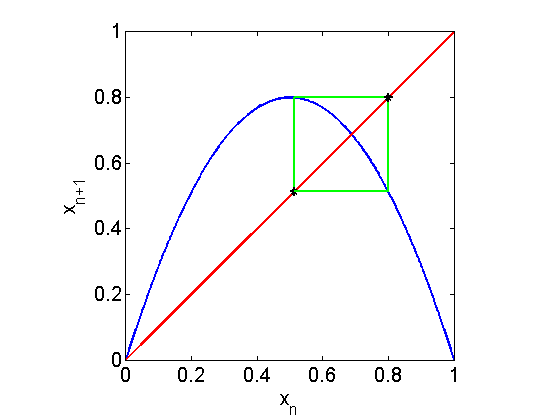
\includegraphics[width=.495\textwidth]{det_cobweb}\hfill
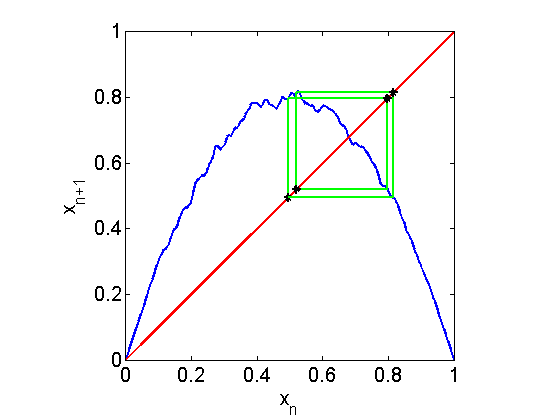
\includegraphics[width=.495\textwidth]{rand_cobweb}
\end{figure}
}
\end{frame}
%------------------------------------------------
\begin{frame}
\misc{ 
Bounds of the Random Logistic Map
\begin{itemize}
\item $\sigma=0.1093,r=2.7,L=0.9,N=112$
\item $\sigma=0.0086,r=3.5,L=0.05,N=200$
\end{itemize}
\begin{figure}[h]
\centering
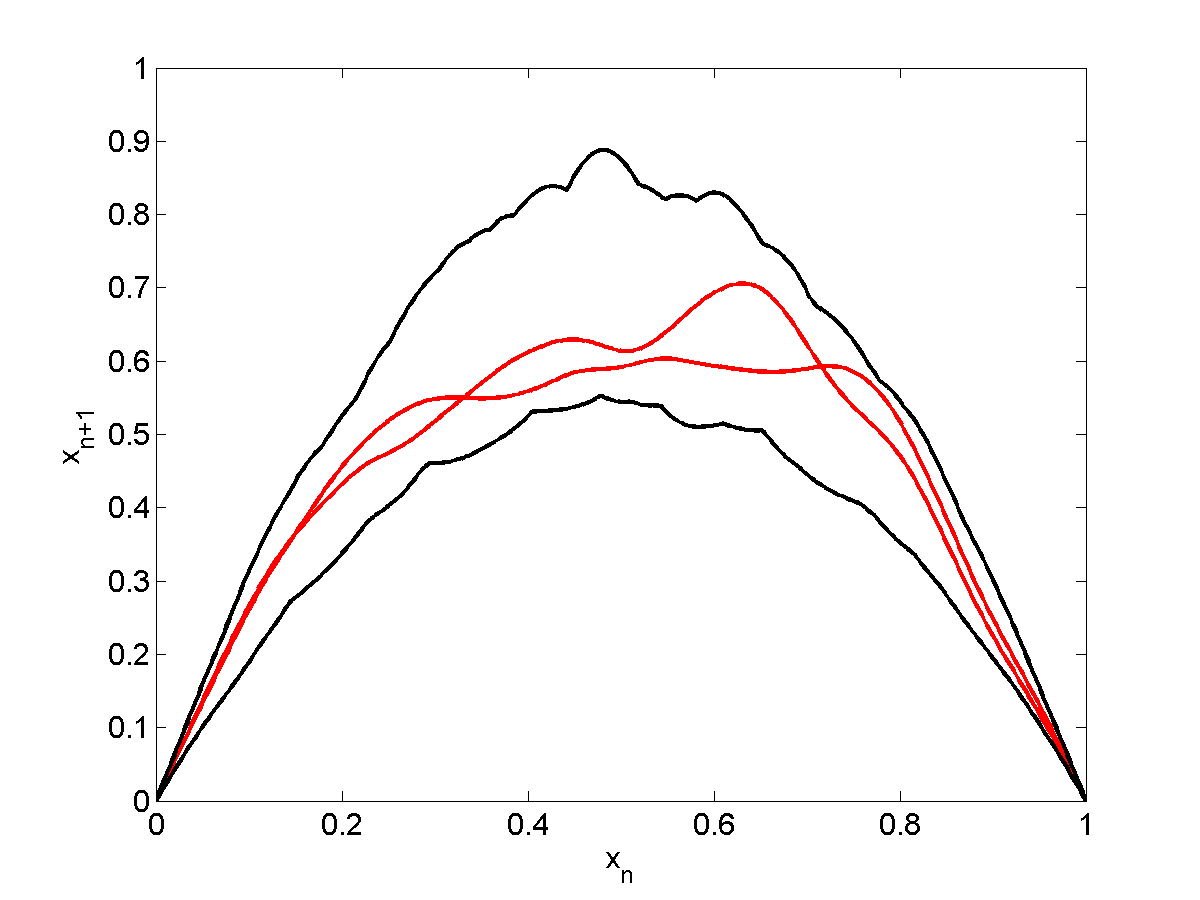
\includegraphics[width=.495\textwidth]{envelope_500_r27_L09}\hfill
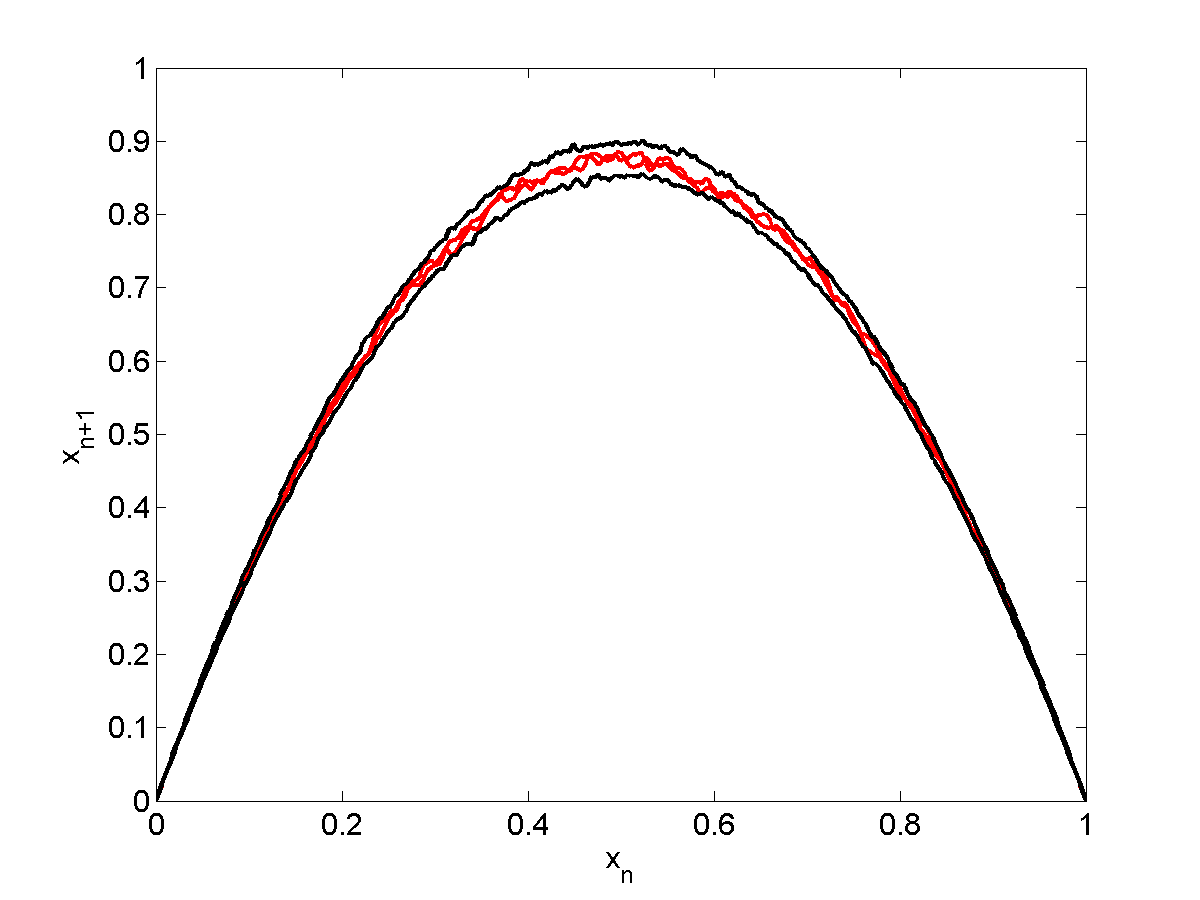
\includegraphics[width=.495\textwidth]{envelope_500_r35_L005}
\end{figure}
}
\end{frame}

%------------------------------------------------

%\fbckg{2.jpg} % Slide background image
\begin{frame}
\misc{Bifurcation Diagram: Logistic Map
\begin{figure}[h]
\centering
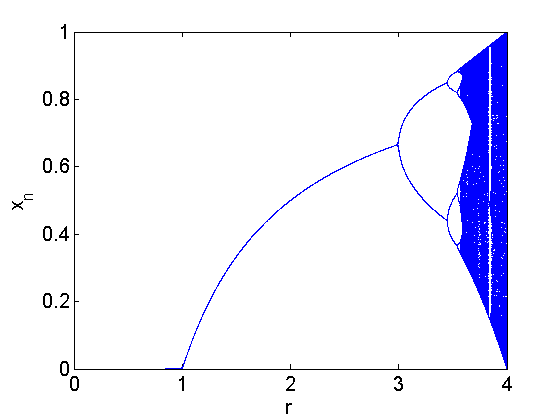
\includegraphics[width=.495\textwidth]{det_bif_1}\hfill
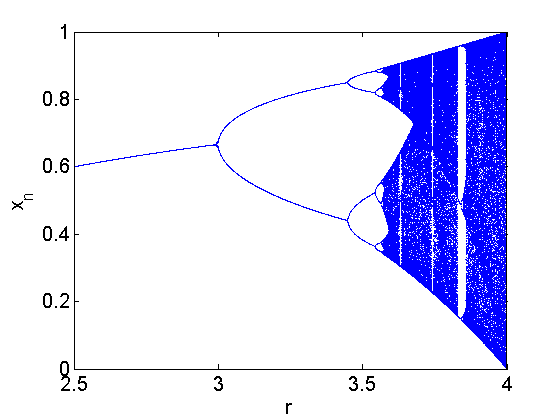
\includegraphics[width=.495\textwidth]{det_bif_2}
\end{figure}
}
\end{frame}
%------------------------------------------------
\fbckg{rlog_bif_L_01} 
\begin{frame}
\end{frame}
%------------------------------------------------

% \fbckg{rlog_bif_zoom_L_01} 
% \begin{frame}
% \end{frame}
%------------------------------------------------

\fbckg{rlog_bif_L_05} 
\begin{frame}
\end{frame}
%------------------------------------------------

% \fbckg{rlog_bif_zoom_L_05} 
% \begin{frame}
% \end{frame}
%------------------------------------------------

\fbckg{rlog_bif_L_09} 
\begin{frame}
\end{frame}
%------------------------------------------------

% \fbckg{rlog_bif_zoom_L_09} 
% \begin{frame}
% \end{frame}
%------------------------------------------------
\fbckg{blank}
\begin{frame}
\misc{ The Lyapunov Exponent
\begin{equation*}
\lambda(x_0) = \lim_{n \to \infty} \frac{1}{n} \sum_{i=0}^{n-1} \ln |f'(x_i)|
\end{equation*}
}
\end{frame}
%------------------------------------------------
\fbckg{blank}
\begin{frame}
\misc{ The Lyapunov Exponent
\begin{itemize}
\item the deterministic map
\item $L=0.1, N = 100, x_0 = 0.7, N_\lambda  =10,000$
\end{itemize}
\begin{figure}[h]
\centering
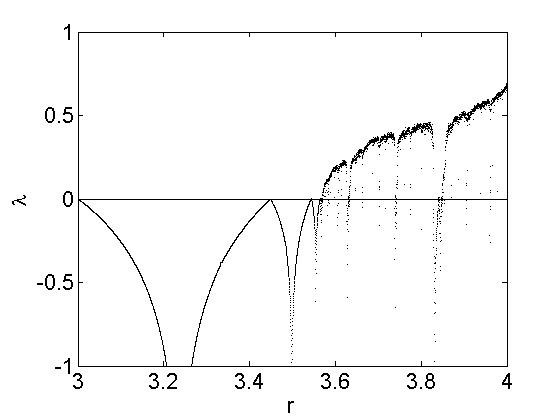
\includegraphics[width=.495\textwidth]{det_log_lyap}\hfill
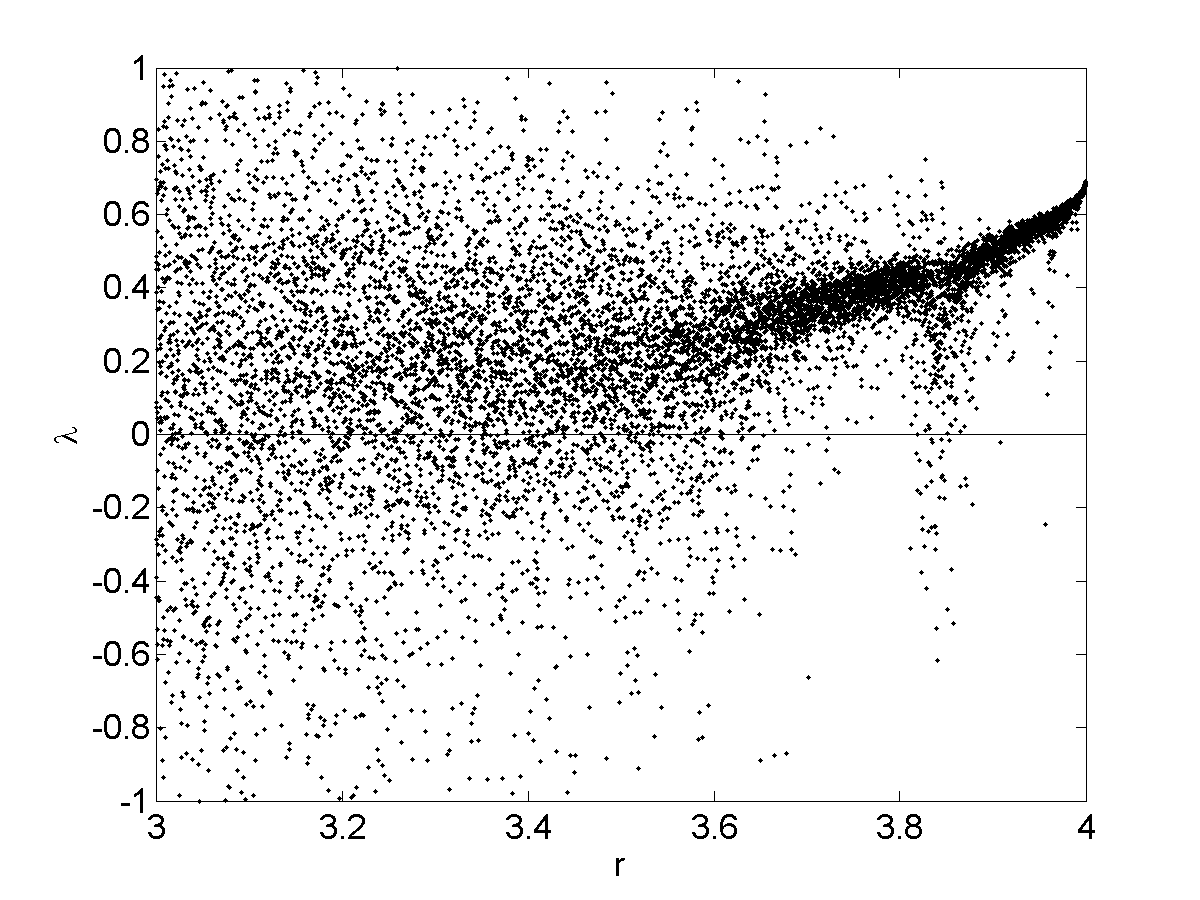
\includegraphics[width=.495\textwidth]{rlog_lyap_L_01}
\end{figure}
}
\end{frame}
%------------------------------------------------
\fbckg{blank}
\begin{frame}
\misc{ The Lyapunov Exponent \\
$L \in \{0.1,0.5,0.9\}, N = 100, x_0 = 0.7, N_\lambda  =10,000$
\begin{figure}[h]
\centering
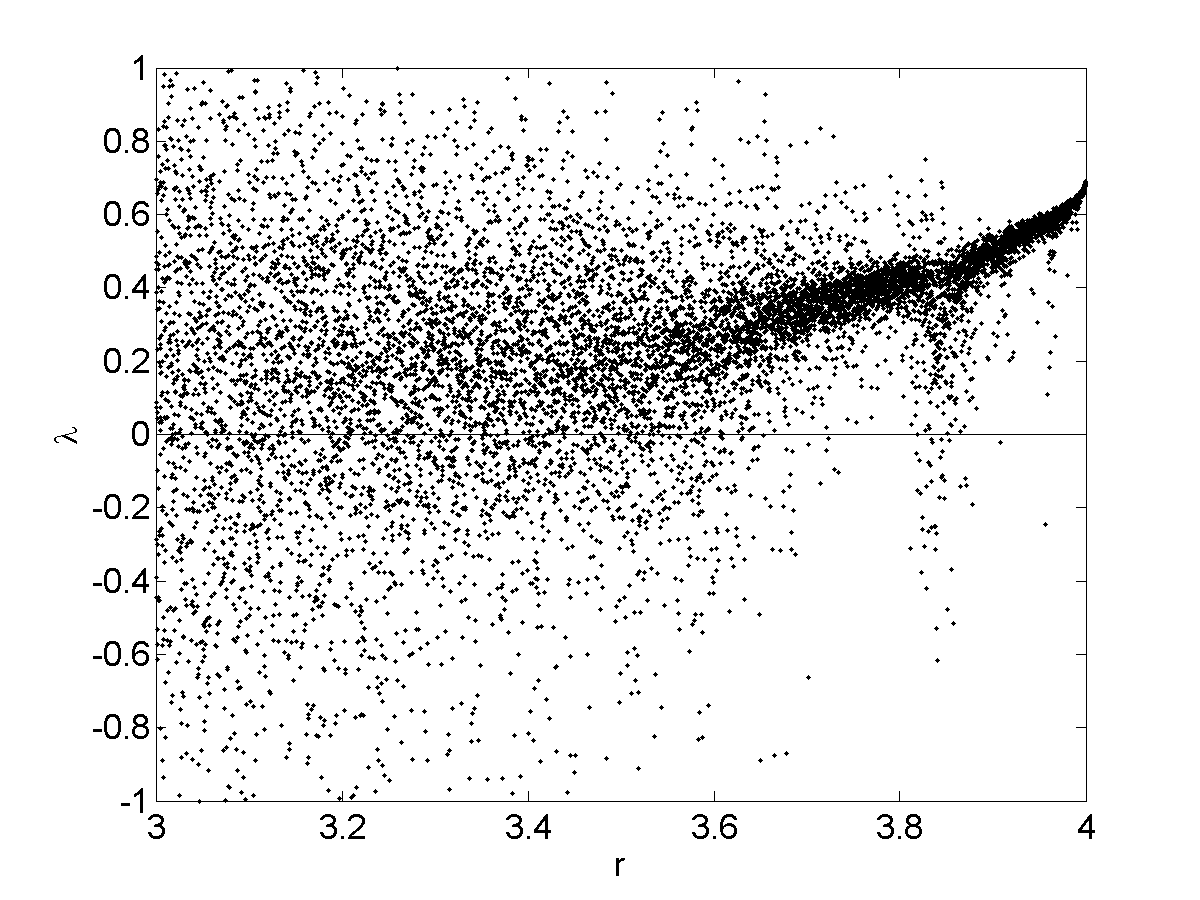
\includegraphics[width=.329\textwidth]{rlog_lyap_L_01}\hfill
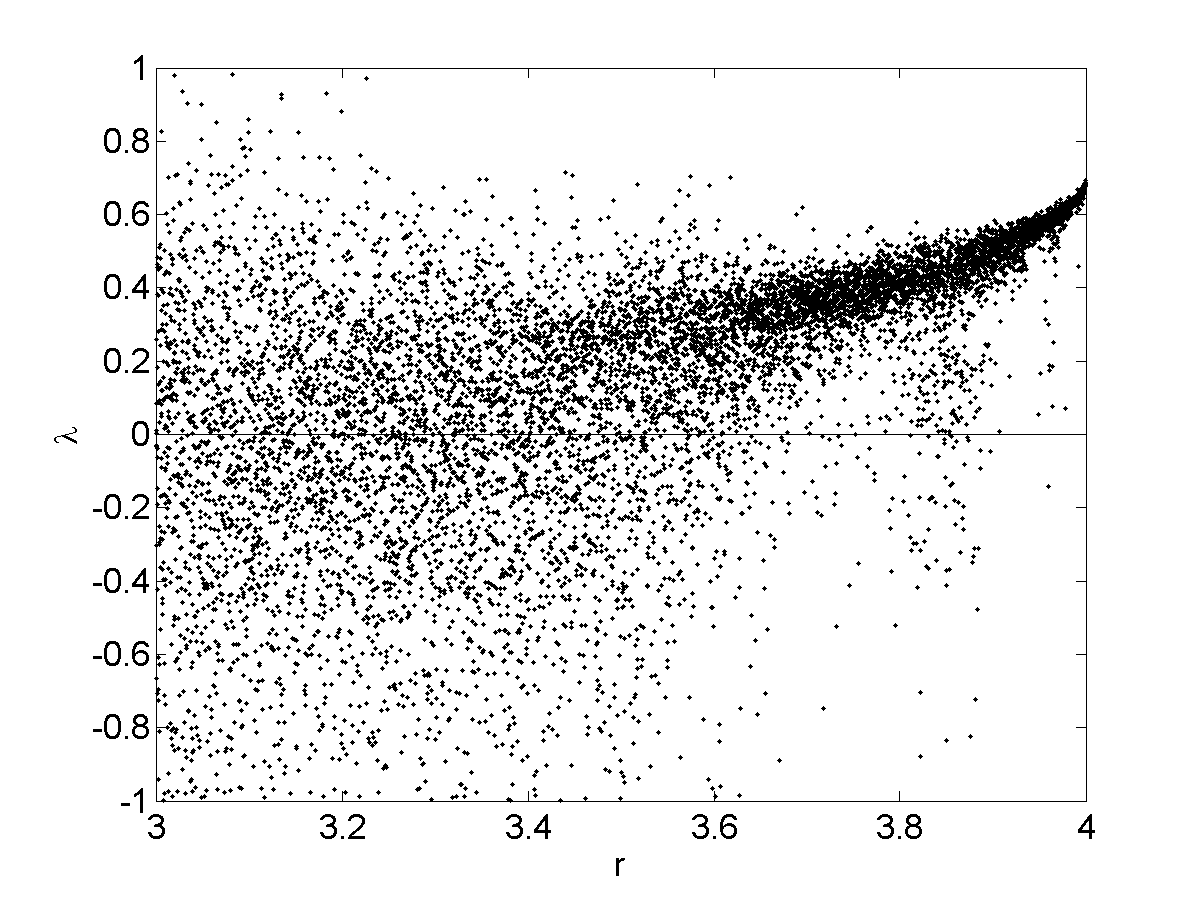
\includegraphics[width=.329\textwidth]{rlog_lyap_L_05}\hfill
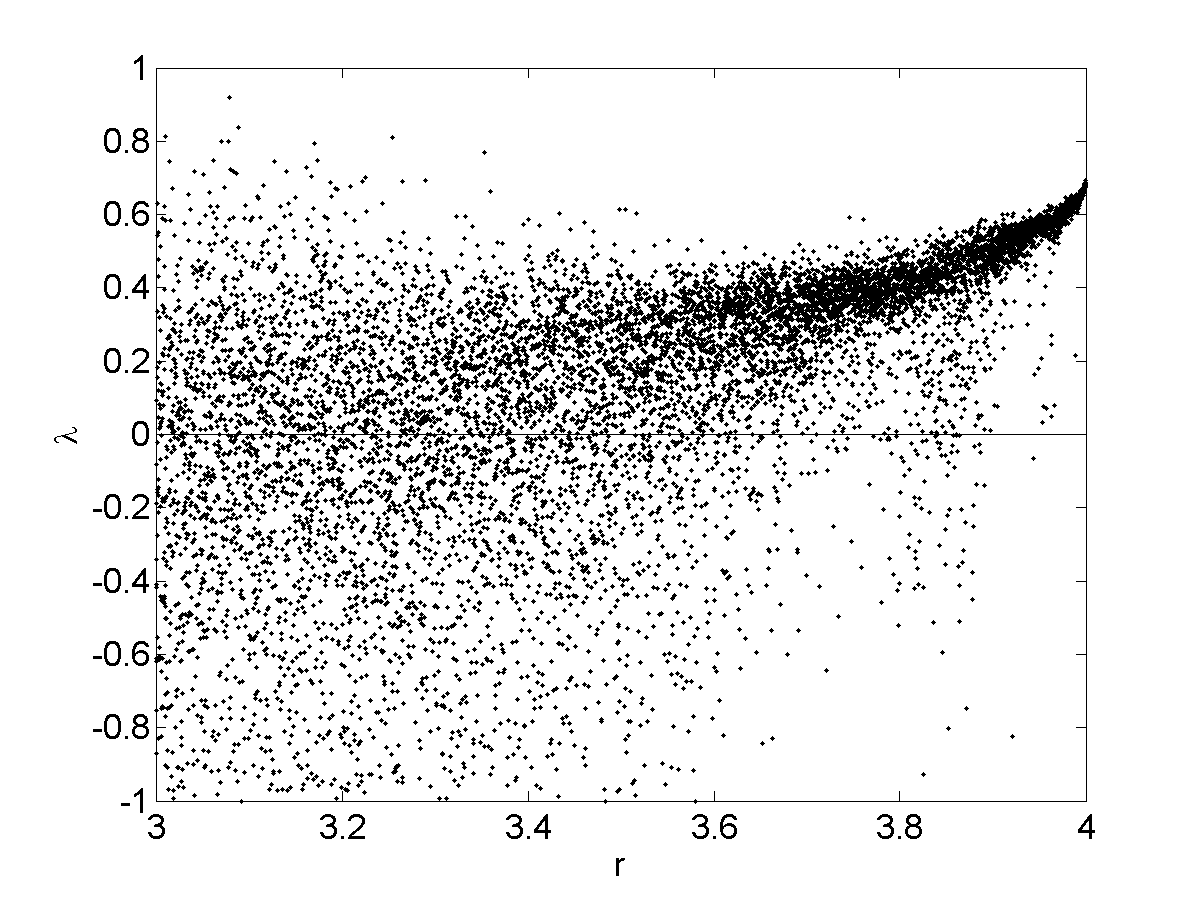
\includegraphics[width=.329\textwidth]{rlog_lyap_L_09}\\
\end{figure}
}
\end{frame}
%------------------------------------------------
\fbckg{blank} % Slide background image
\begin{frame}
\misc{\pitem{Long correlation length $\to$ wider range of
    randomness, lower density of stable orbits} \pitem{Stabilizing effect on the logistic map}
  \pitem{Preservation of some features of Lyapunov exponents}
  \fitem{Noise is not log-normal}} 
\end{frame}

%------------------------------------------------

\fbckg{blank}
\begin{frame}
\framedsl{Circle Map} % Text in this environment will be made large, uppercase and will wrap multiple lines
\misc{
\begin{align*}
\begin{split}
x_{n+1}= F_c(x_n) &=  x_n + \omega - \frac{k}{2\pi}\sin(2\pi x_n)\\
f_c(x_n) &= x_n + 2\pi \omega - \frac{k}{2\pi}\sin(2\pi x_n) \mod 1\\
\omega \in [0,1] &\>, k \in \mathbb{R}  
\end{split}
\end{align*}
}
\end{frame}

%------------------------------------------------
\begin{frame}
\misc{ Orbit Diagrams\\
\begin{itemize}
\item Deterministic circle map for $x_0=0.8,k=1,\omega=0.3$
\item $\hat{\xi}_n \sim Unif(-M_n,M_n), x_0=0.8, \omega = 0.3, k=1, \alpha = 10^{-5},L=0.1, N=100$
\item $\hat{\xi}_n \sim N(0,\hat{\sigma}_n^2), x_0=0.8,\omega = 0.3, k=1, \alpha = 10^{-5},L=0.1, N=100$
\end{itemize}
\begin{figure}[h]
\centering
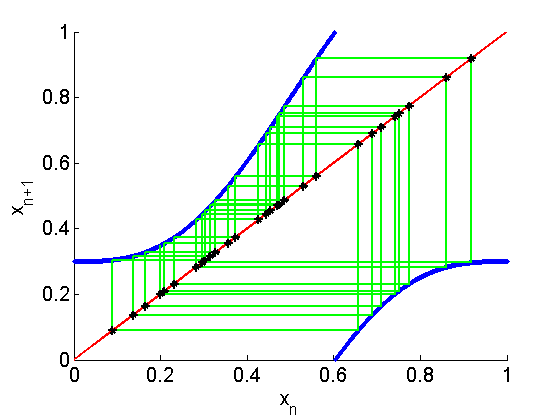
\includegraphics[width=.329\textwidth]{detcirc_cobweb}\hfill
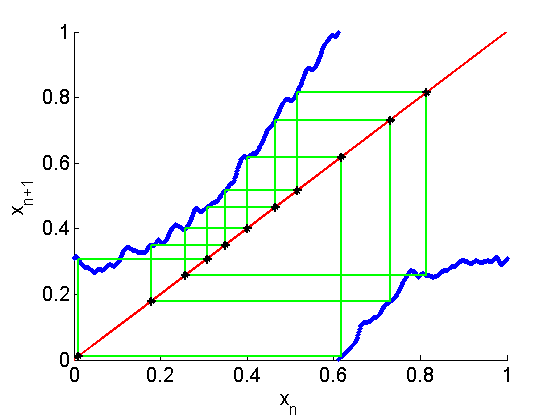
\includegraphics[width=.329\textwidth]{randcirc_cobweb}\hfill
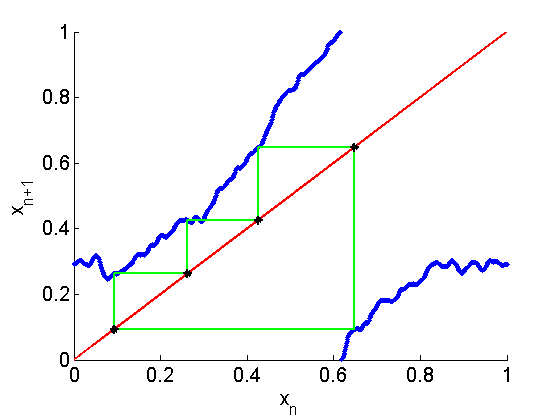
\includegraphics[width=.329\textwidth]{randcirc_norm_cobweb}\hfill
\end{figure}
}
\end{frame}
%------------------------------------------------
\begin{frame}
\misc{ 
Bounds of the Random Circle Map
\begin{itemize}
\item $L=0.5,\alpha = 10^{-5},k=1.5,\omega=0.3,N=100$
\item $L=0.1,\alpha = 10^{-5},k=1.5,\omega=0.7,N=100$
\end{itemize}
\begin{figure}[h]
\centering
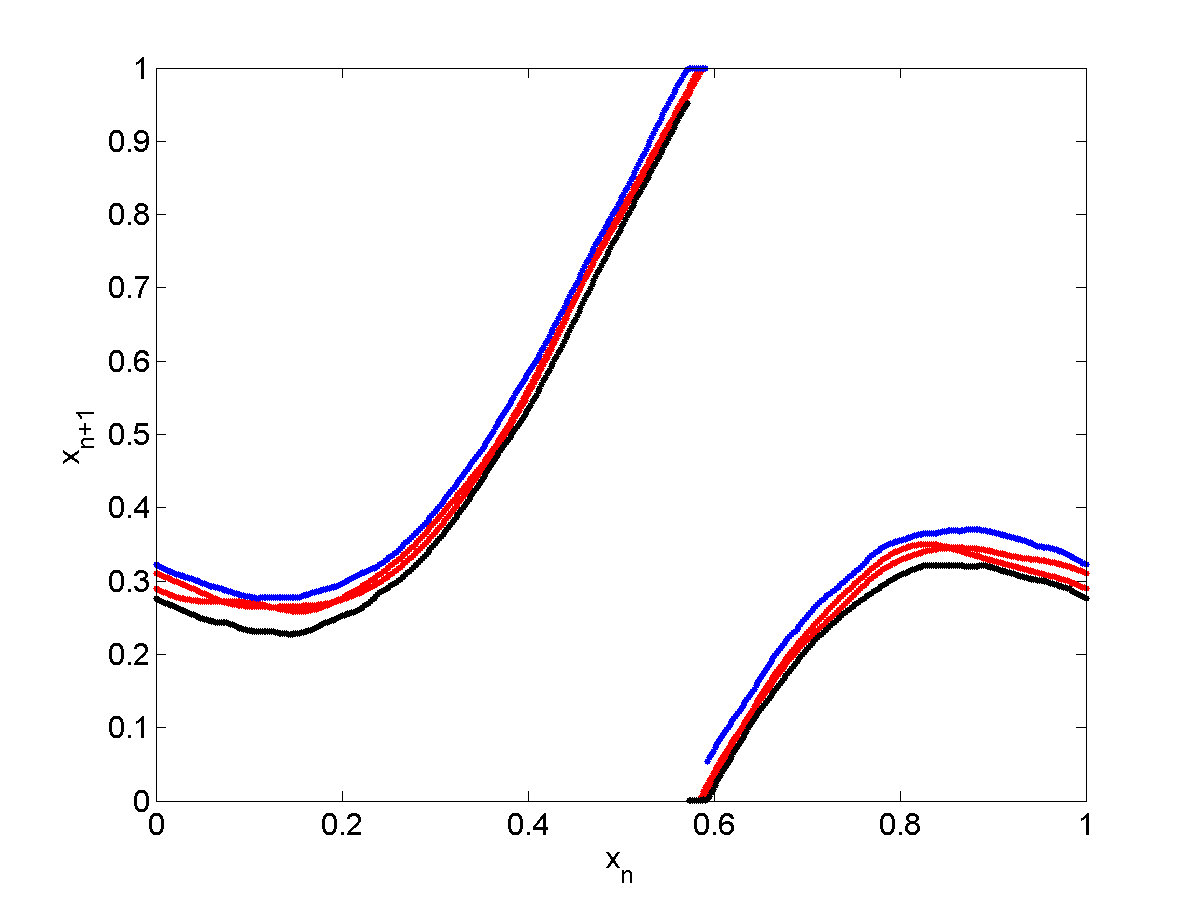
\includegraphics[width=.495\textwidth]{envelope_norm_500_k15_L05_w03}\hfill
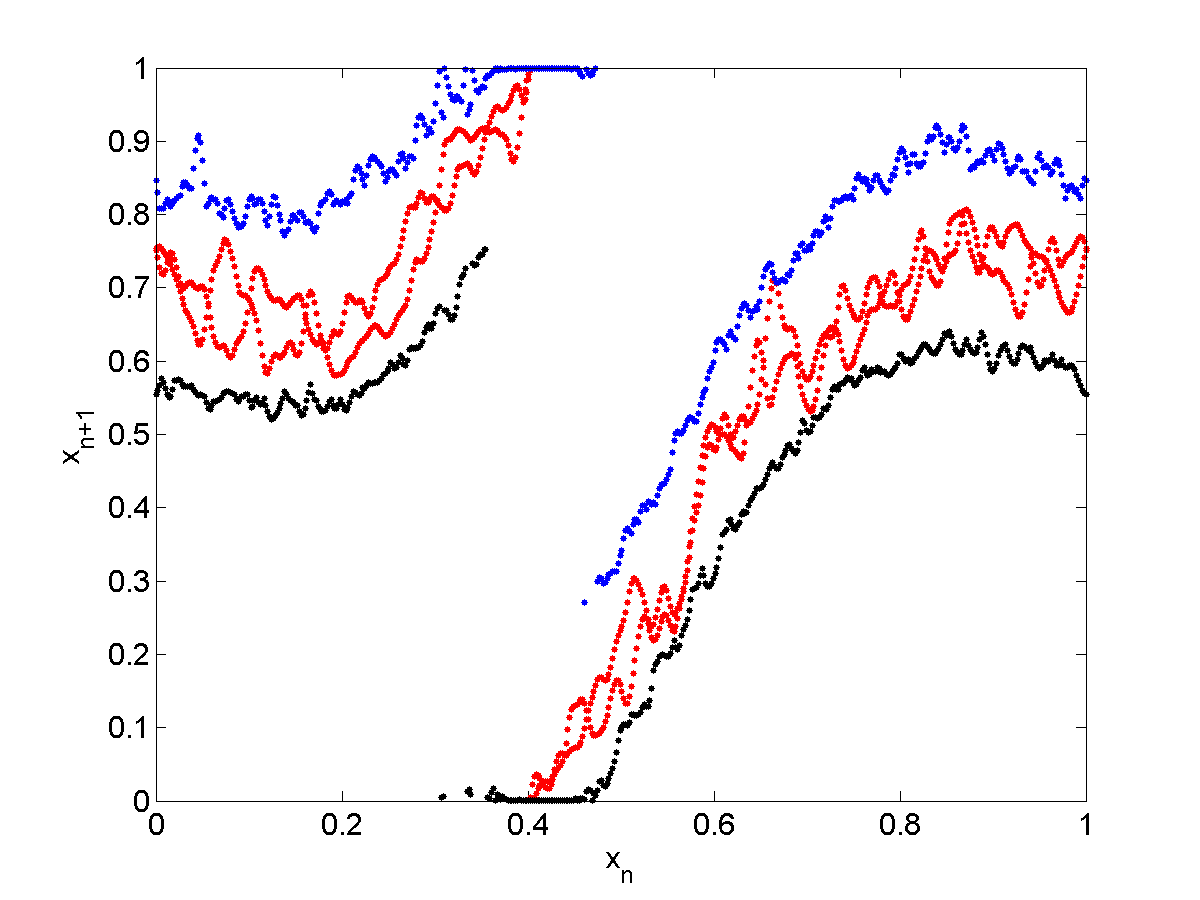
\includegraphics[width=.495\textwidth]{envelope_norm_500_k15_L01_w07}
\end{figure}
}
\end{frame}

%------------------------------------------------

\begin{frame}
\misc{ The Arnold Tongues\\
$\omega \in [0,1], \Delta \omega = 0.001, k \in [0,1.5],\Delta k = 0.0015, p_{max}=100$
\begin{figure}[h]
\centering
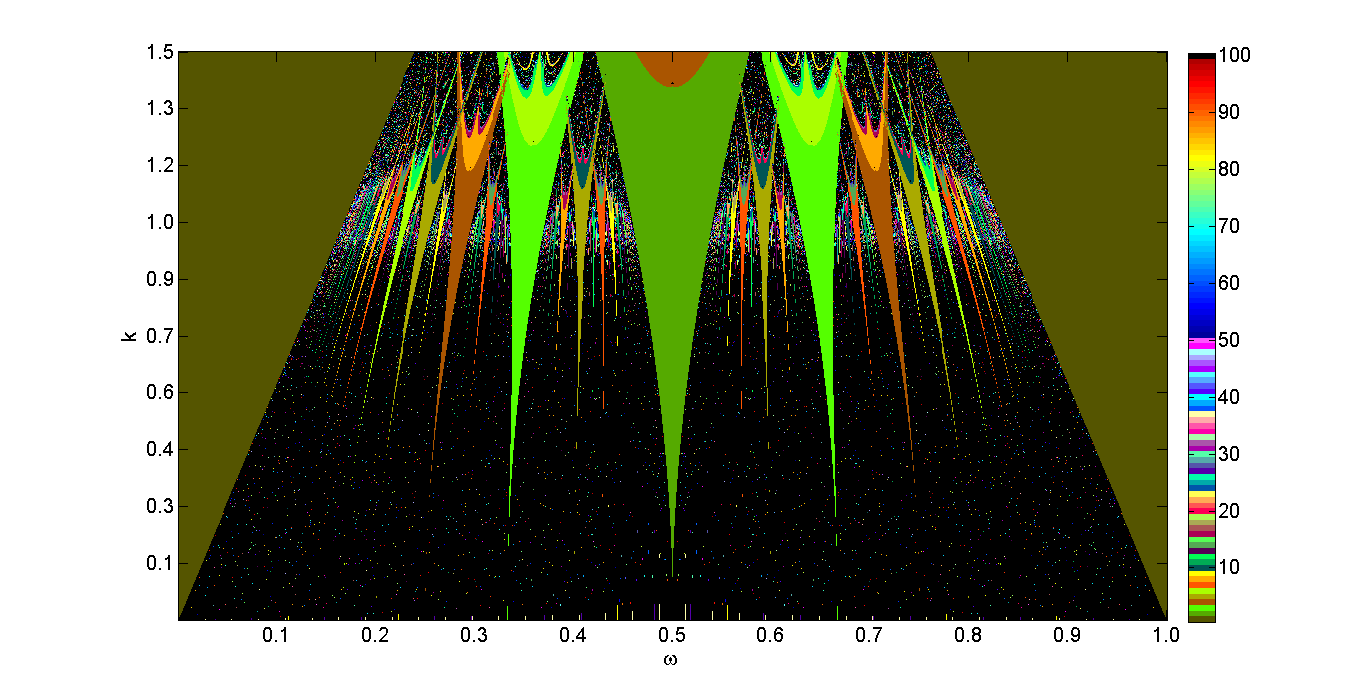
\includegraphics[scale=0.28]{tongues_1000_det}
\end{figure}
}
\end{frame}
%------------------------------------------------
\fbckg{tongues_norm_1000_L_01} 
\begin{frame}
\end{frame}
%------------------------------------------------
\fbckg{tongues_norm_1000_L_05} 
\begin{frame}
\end{frame}
%------------------------------------------------
\fbckg{tongues_norm_1000_L_09} 
\begin{frame}
\end{frame}

%------------------------------------------------
\fbckg{blank} 
\begin{frame}
\misc{ Rotation Number\\
$\rho(f)$ is the fractional part of 
\begin{equation*}
\rho_0(F) = \lim_{n \to \infty} \frac{|F^n(x)|}{n}
\end{equation*}
for any lift $F$ of $f$. That is, $\rho(f)$ is the unique
number in [0,1) such that $\rho_0(F)-\rho(f)$ is an integer.
}
\end{frame}
%------------------------------------------------
\begin{frame}
\misc{ The Devil's Staircase\\
$\omega \in [0,1],\Delta \omega = 0.001$
\begin{figure}[h]
\centering
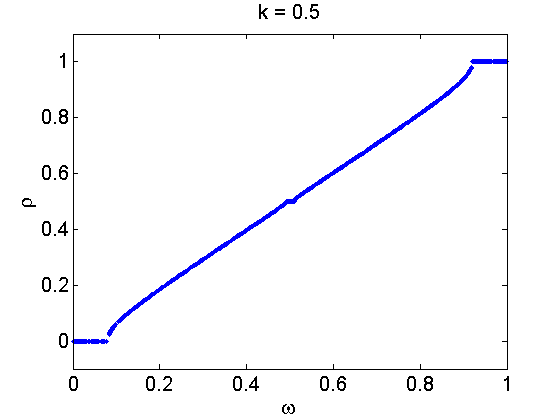
\includegraphics[width=.329\textwidth]{detcirc_devil_k05}\hfill
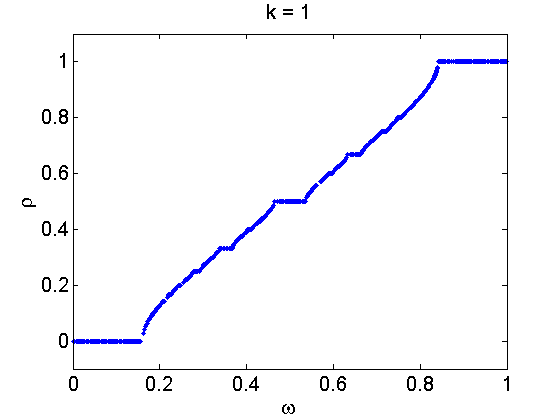
\includegraphics[width=.329\textwidth]{detcirc_devil_k1}\hfill
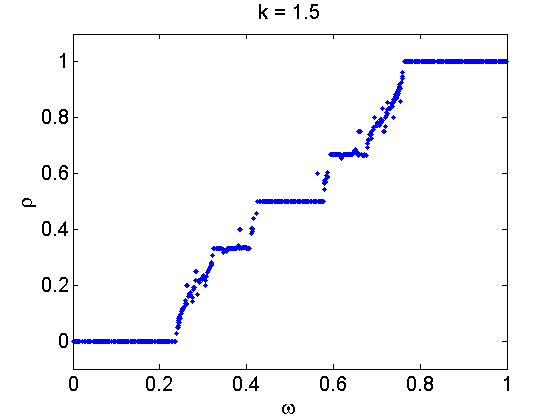
\includegraphics[width=.329\textwidth]{detcirc_devil_k15}
\end{figure}
}
\end{frame}
%------------------------------------------------
\begin{frame}
\misc{ The Devil's Staircase\\
$\alpha = 10^{-5},L=0.05, N=200,\Delta \omega = 0.0001$
\begin{figure}[h]
\centering
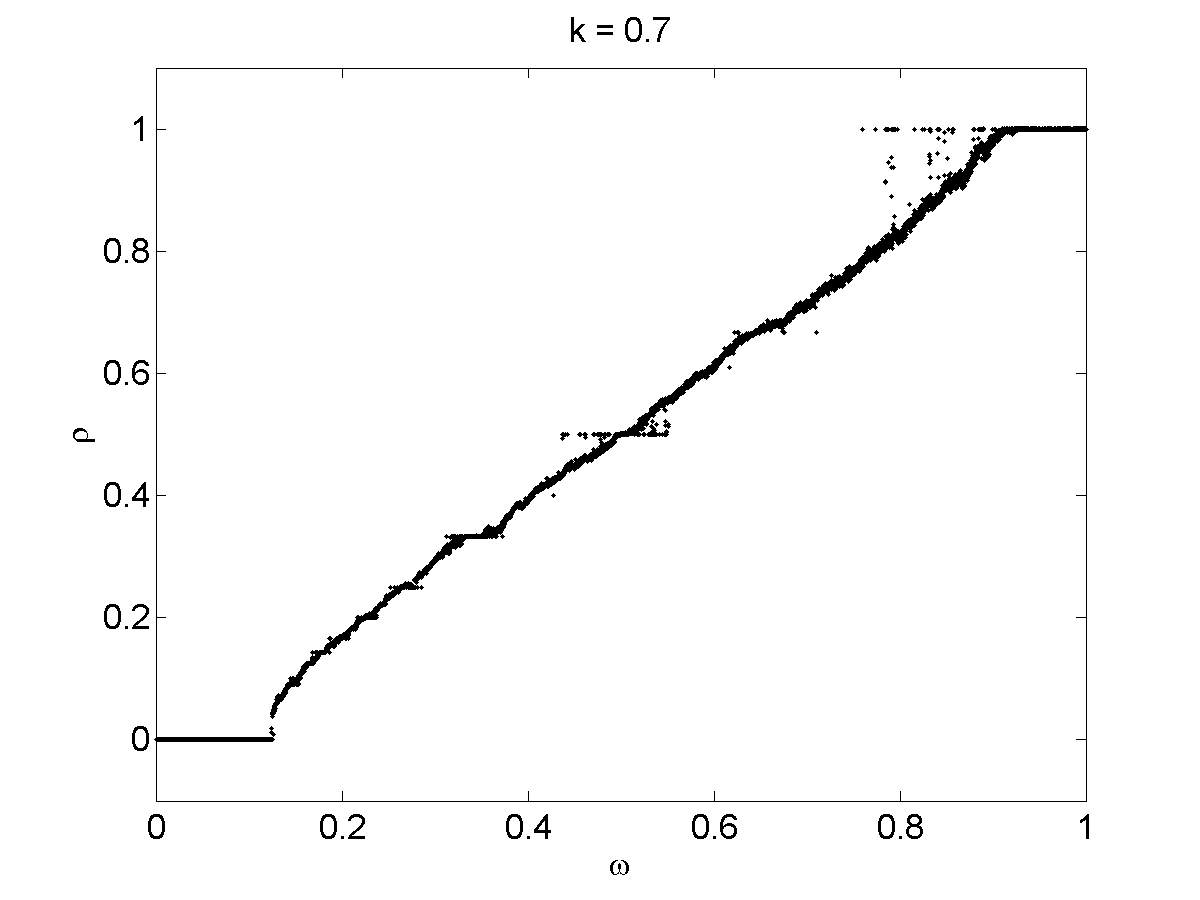
\includegraphics[width=.329\textwidth]{rcirc_n_devil_k07_L005}\hfill
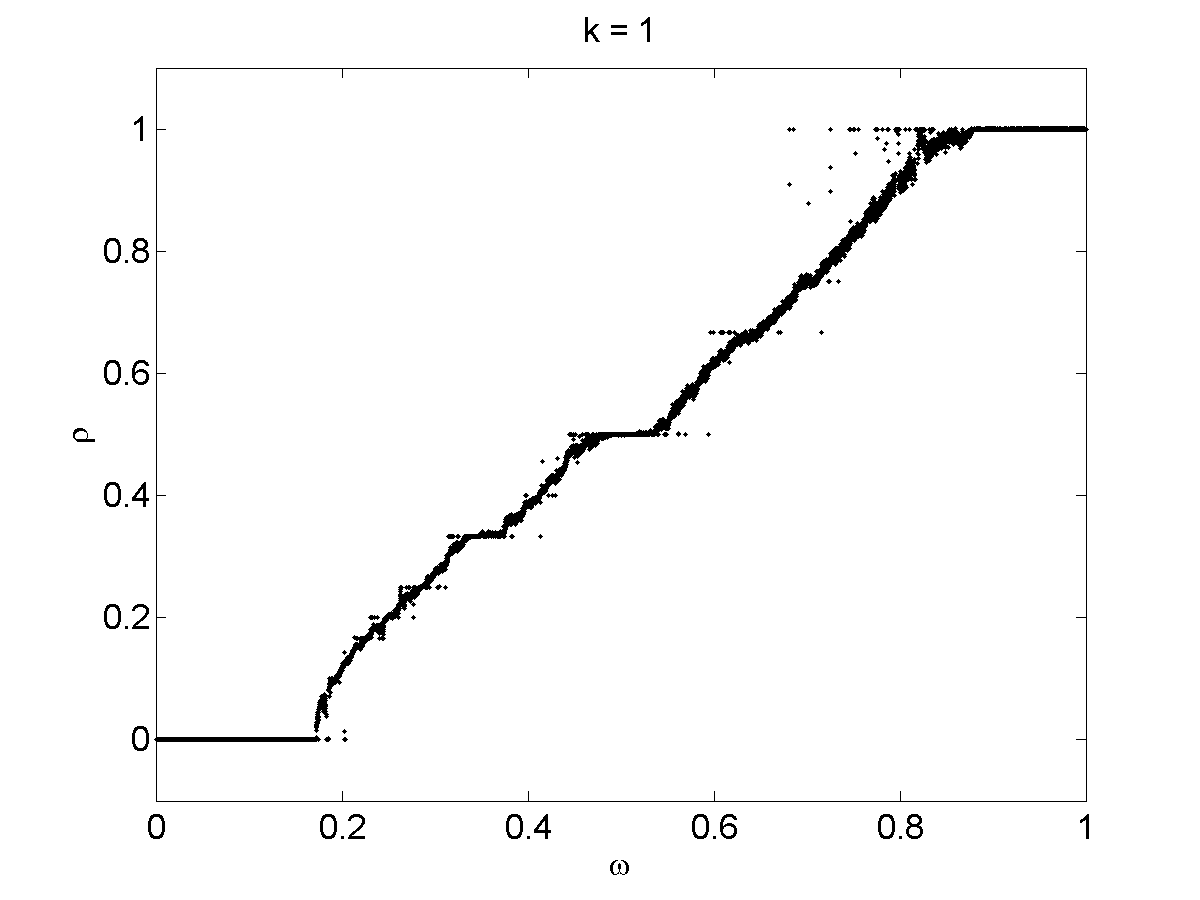
\includegraphics[width=.329\textwidth]{rcirc_n_devil_k1_L005}\hfill
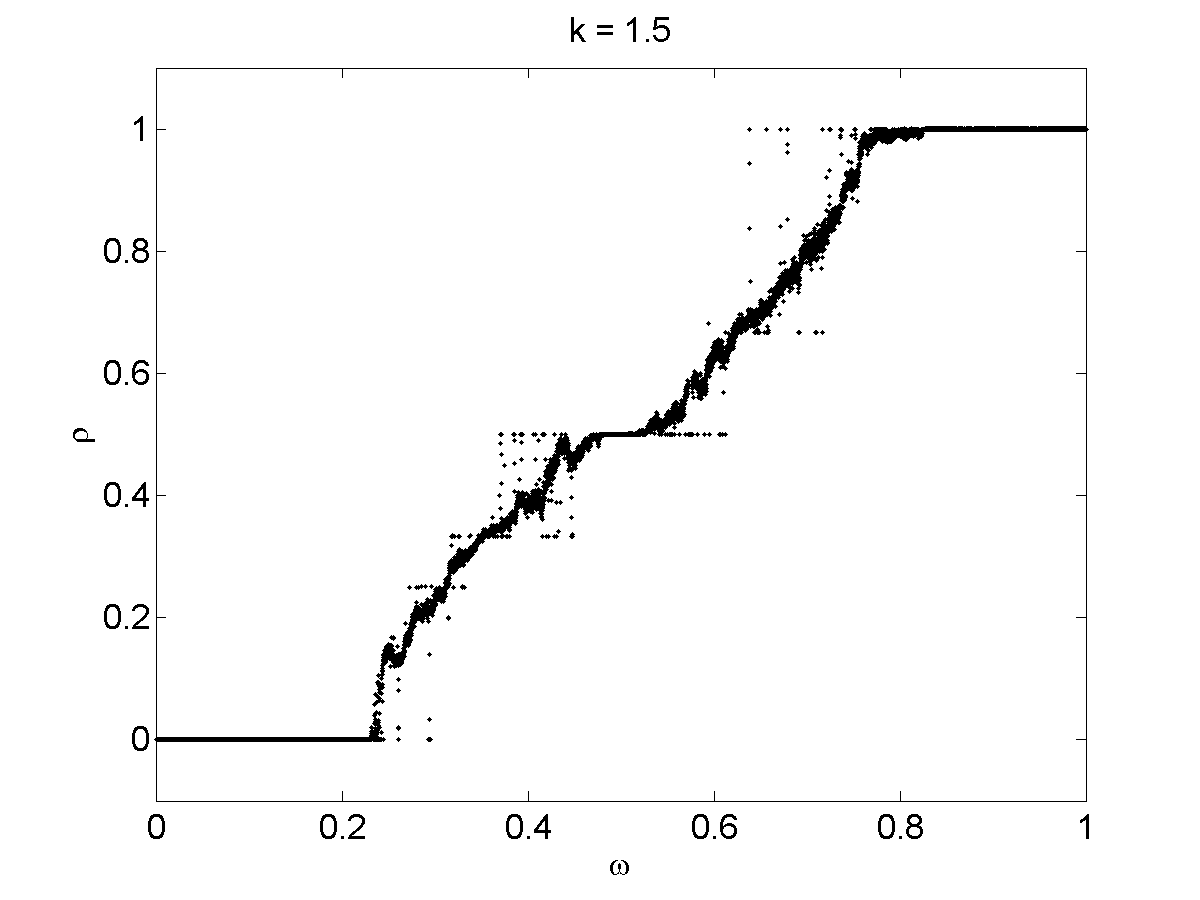
\includegraphics[width=.329\textwidth]{rcirc_n_devil_k15_L005}
\end{figure}
}
\end{frame}
%------------------------------------------------
% \fbckg{blank}
% \begin{frame}
% \misc{ Histogram of rotation numbers in the random circle map\\
% $L=0.1$, $k=1$, $\alpha = 10^{-5}$,$\omega = 0.45$,$N_{sim}=1000$ 
% \begin{figure}
% \centering
% 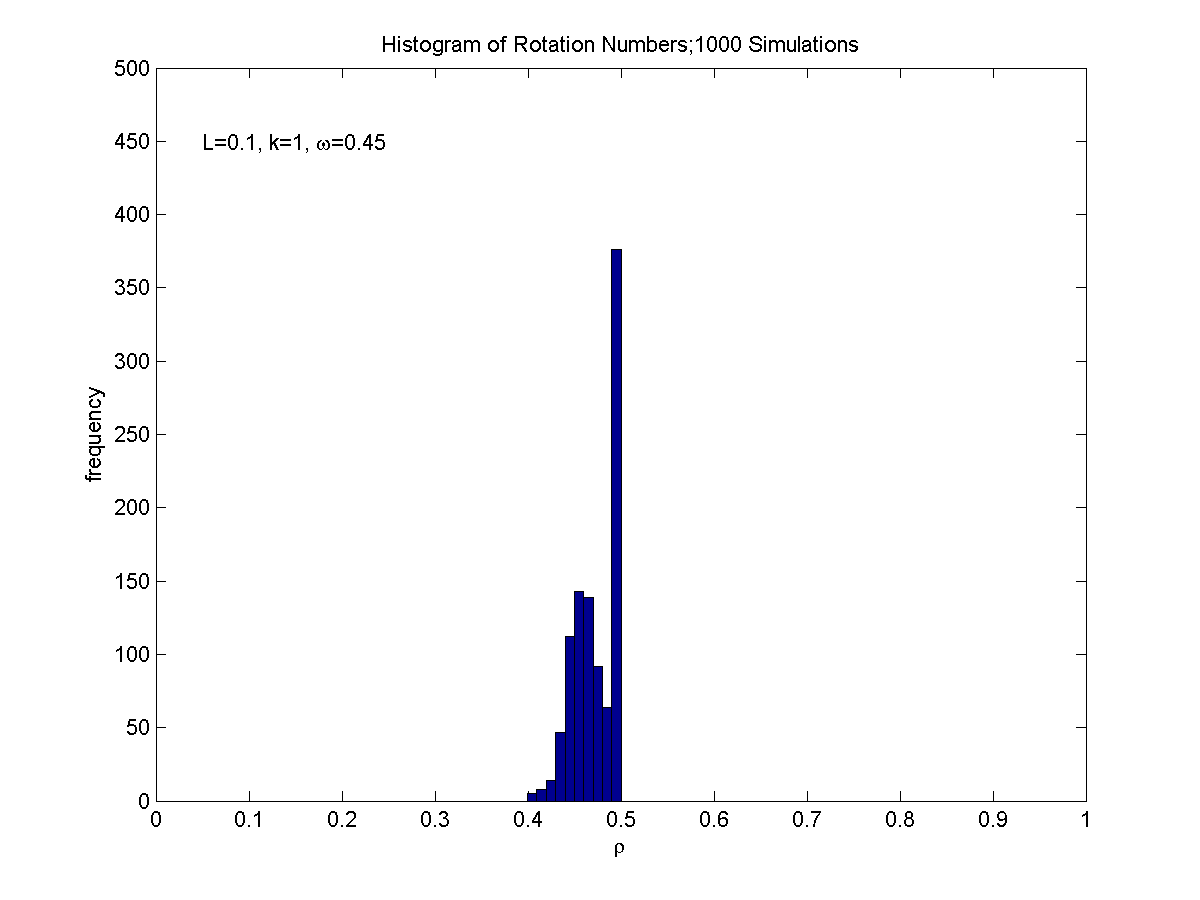
\includegraphics[width=.495\textwidth]{hist_rho_k1_L01_om045}\hfill
% 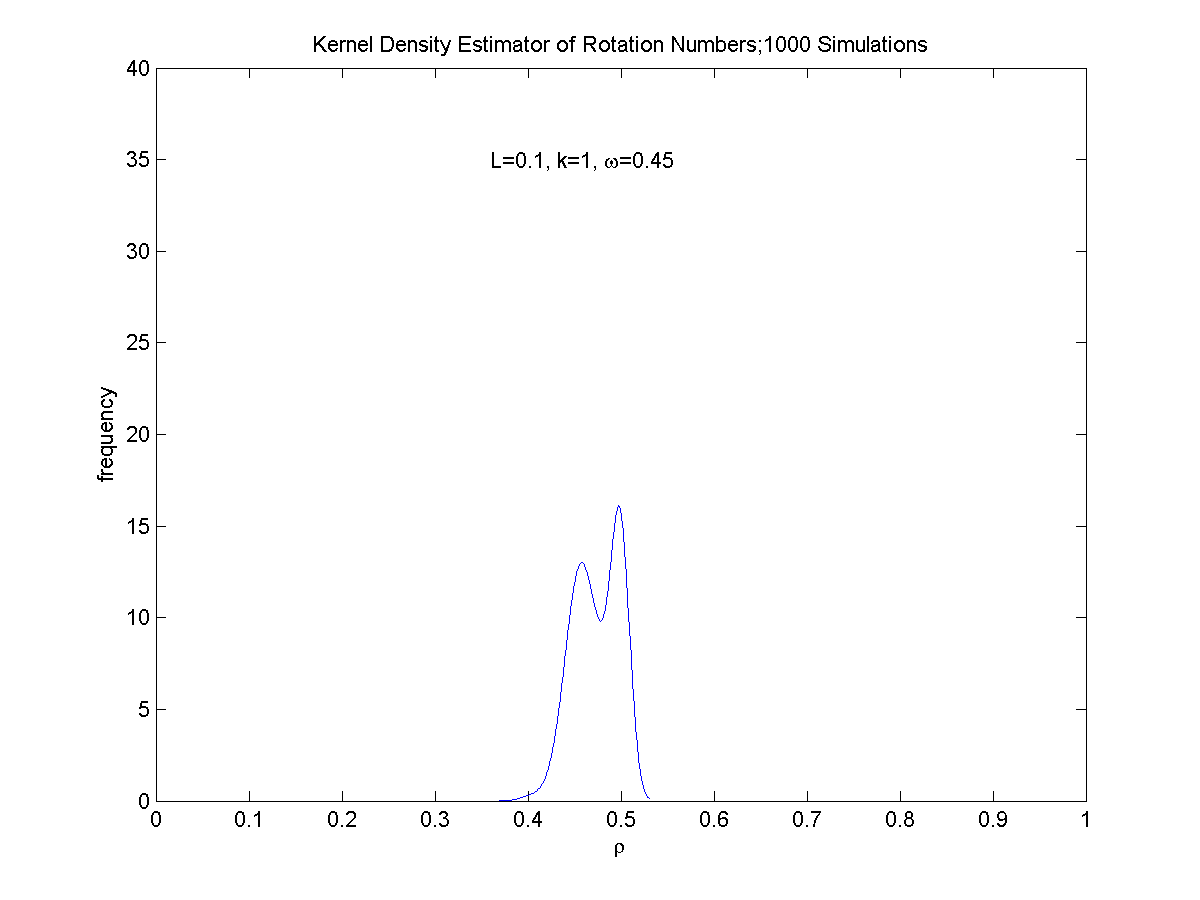
\includegraphics[width=.495\textwidth]{kde_rho_k1_L01_om045}
% \end{figure}
% }
% \end{frame}

%------------------------------------------------
\fbckg{blank}
\begin{frame}
\misc{ The Lyapunov Exponent 
\begin{figure}[h]
\centering
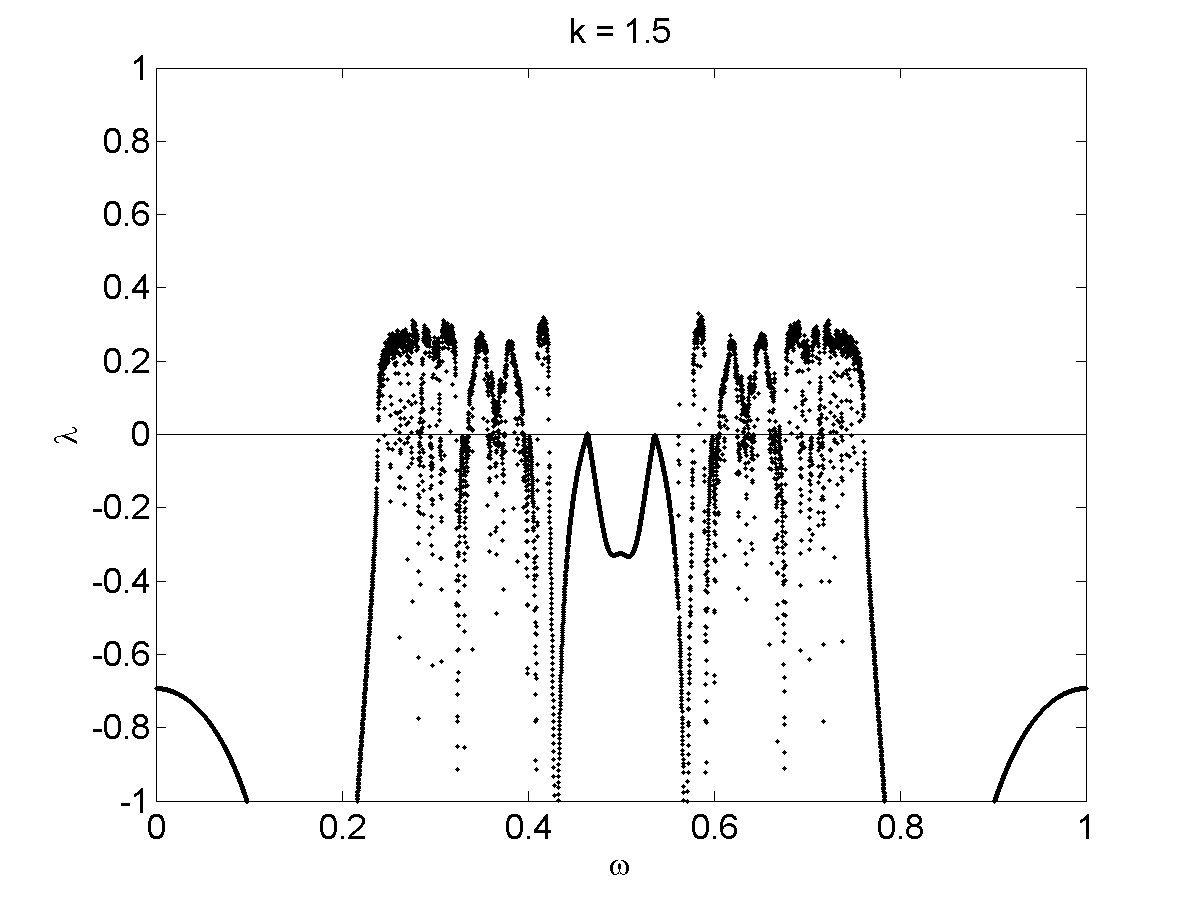
\includegraphics[width=.495\textwidth]{detcirc_lyap_10000_k_15_w}\hfill
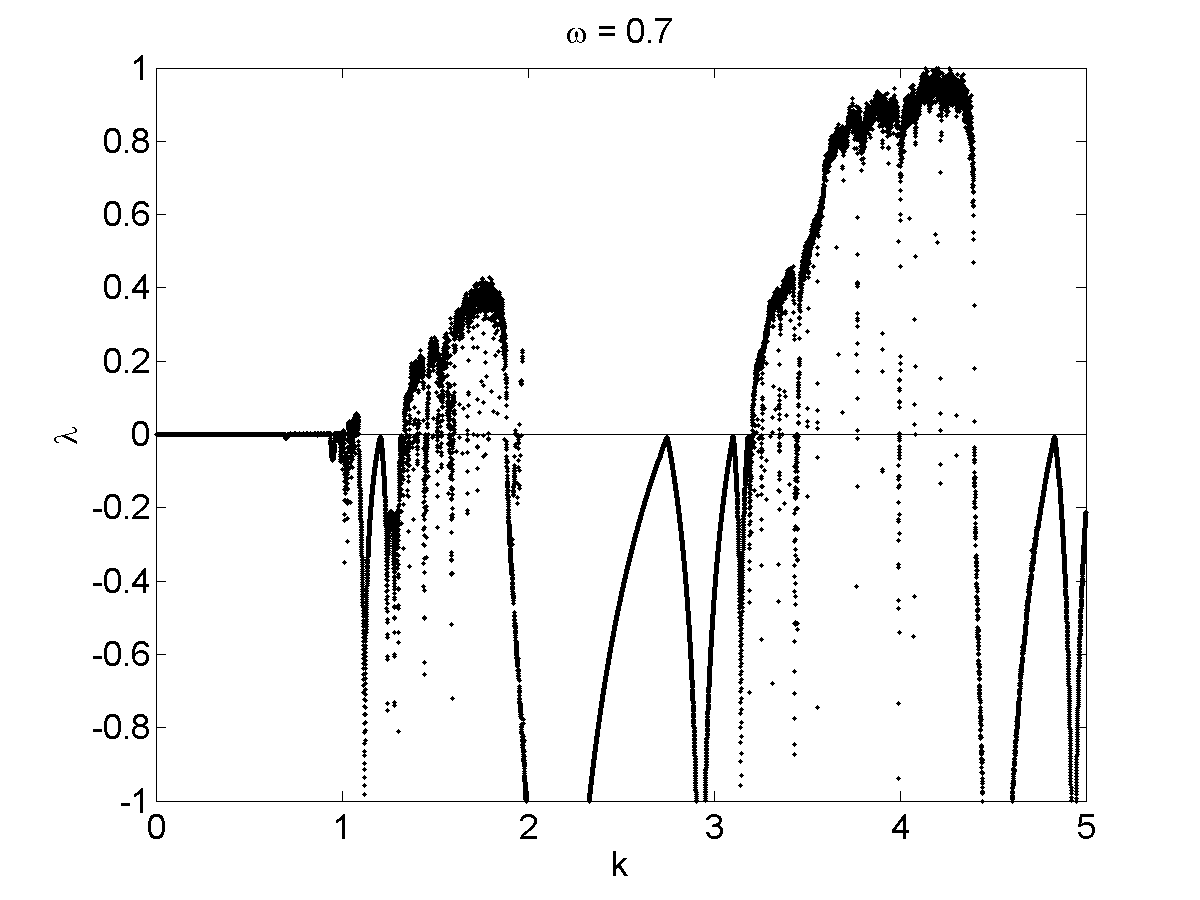
\includegraphics[width=.495\textwidth]{det_circ_lyap_k}
\end{figure}
}
\end{frame}
%------------------------------------------------
\begin{frame}
\misc{ The Lyapunov Exponent 
\begin{itemize}
\item $L=0.1, N = 100, \alpha = 10^{-5}, N_\lambda = 10,000$
\item $L=0.9, N = 100, \alpha = 10^{-5}, N_\lambda = 10,000$
\end{itemize}
\begin{figure}[h]
\centering
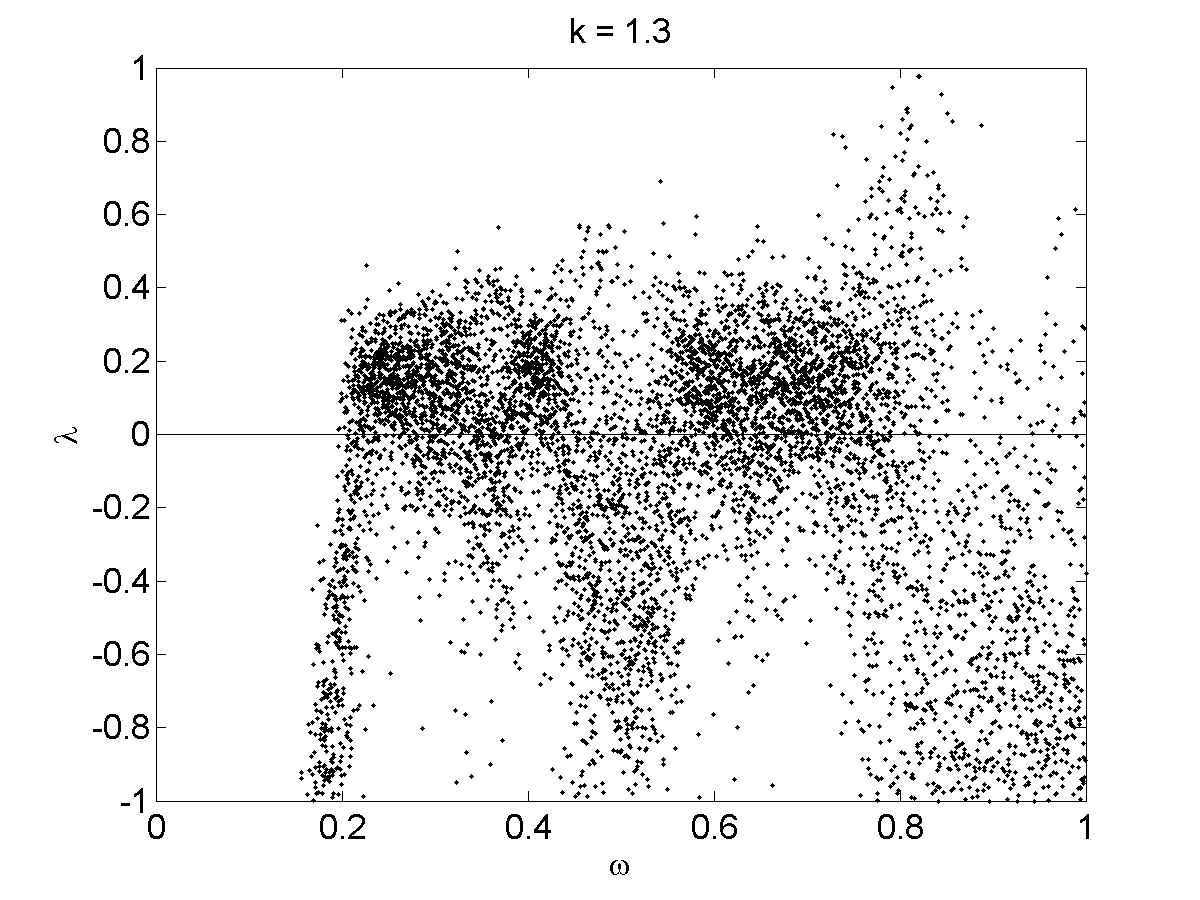
\includegraphics[width=.495\textwidth]{rcirc_n_lyap_10000_L_01_k_13_w}\hfill
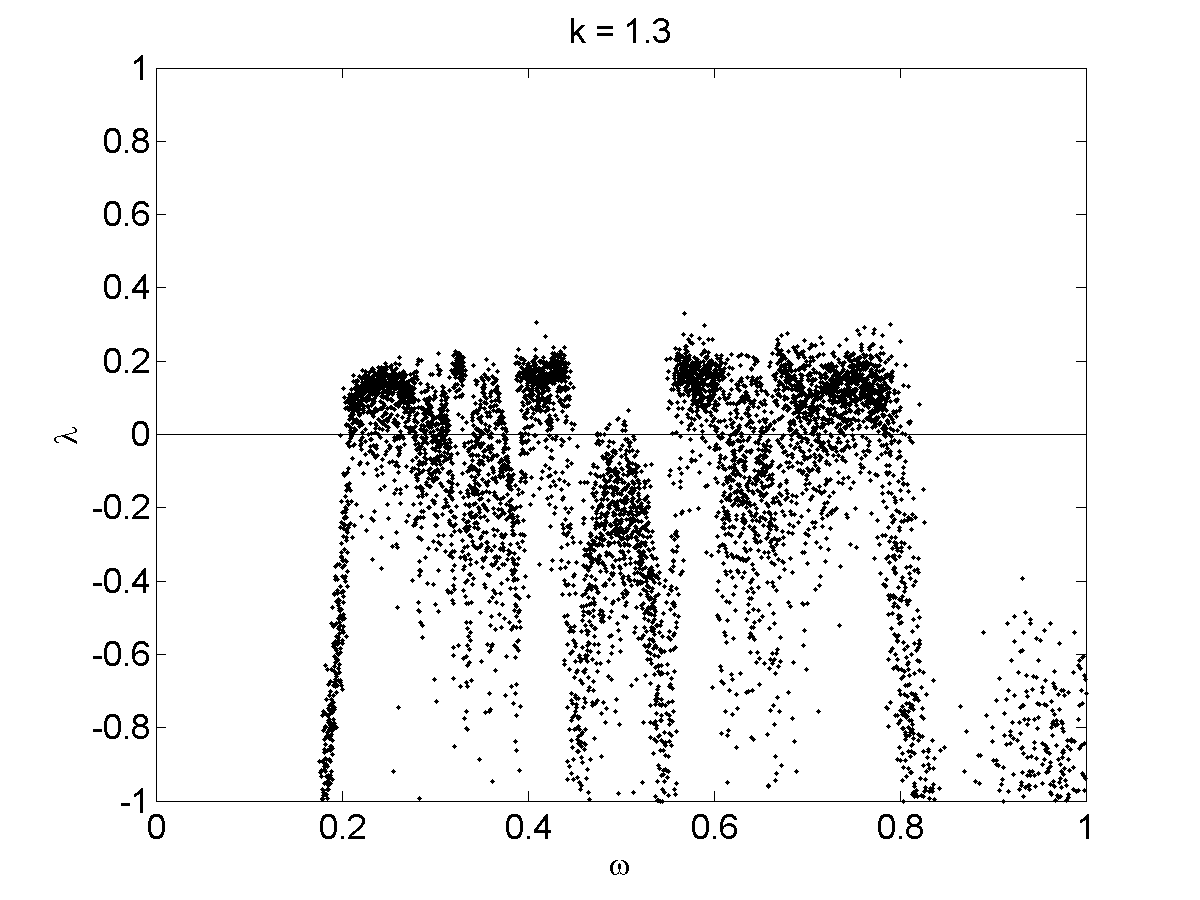
\includegraphics[width=.495\textwidth]{rcirc_n_lyap_10000_L_09_k_13_w}
\end{figure}
}
\end{frame}
%------------------------------------------------
\begin{frame}
\misc{ The Lyapunov Exponent 
\begin{itemize}
\item $L=0.1, N = 100, \alpha = 10^{-5}, N_\lambda = 10,000$
\item $L=0.9, N = 100, \alpha = 10^{-5}, N_\lambda = 10,000$
\end{itemize}
\begin{figure}[h]
\centering
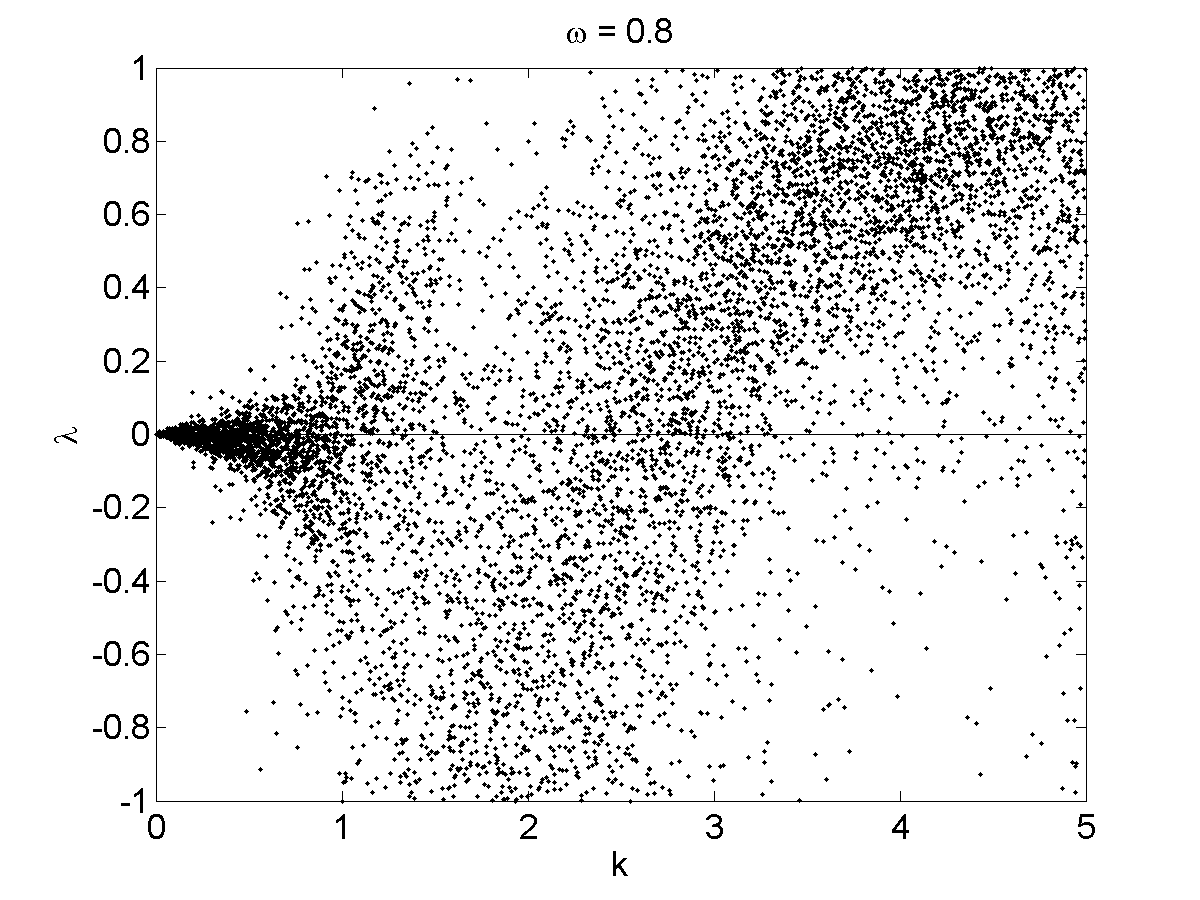
\includegraphics[width=.495\textwidth]{rcirc_n_lyap_10000_L_01_w_08_k}\hfill
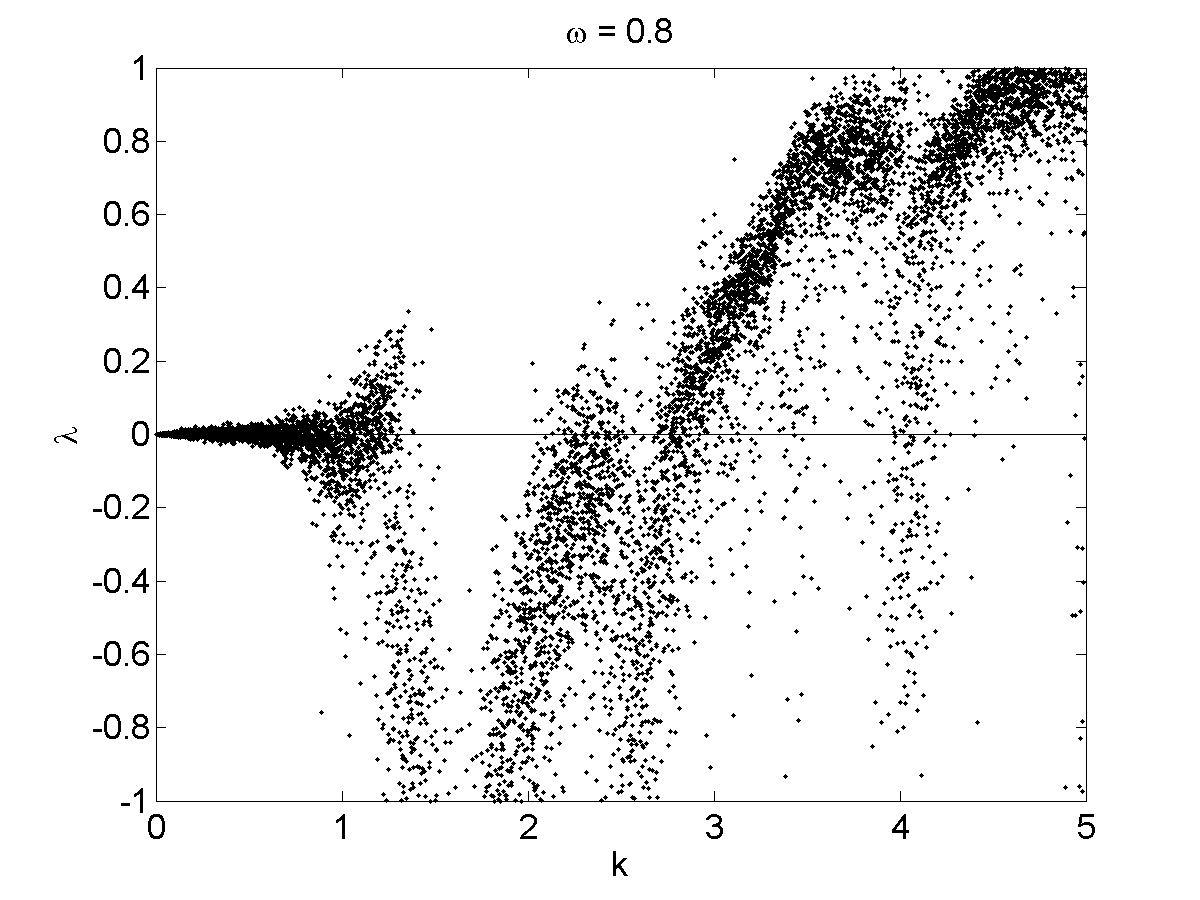
\includegraphics[width=.495\textwidth]{rcirc_n_lyap_10000_L_09_w_08_k}
\end{figure}
}
\end{frame}
%------------------------------------------------

\fbckg{blank} % Slide background image
\begin{frame}
\misc{\pitem{Short correlation length $\to$ wider range of
    randomness} \pitem{Destabilizing effect on the circle map}
  \pitem{Noisy rotation numbers} \pitem{Preservation of some features
    of Lyapunov exponents} \fitem{Log-normal noise}} 
\end{frame}
%------------------------------------------------
\begin{frame}
\pointedsl{\large Effect of noise on remediation} % Text in this environment is printed in a 
\end{frame}
%------------------------------------------------
\fbckg{blank} % Slide background image
\begin{frame}
\misc{\pitem{Log-normal noise: destabilizing effect $\to$ chaotic
    behavior $\to$ well mixed solutions }
\fitem{Non log-normal noise: stabilizing effect $\to$ less well mixed solutions} } 
\end{frame}

%------------------------------------------------

%\fbckg{1.jpg} % Slide background image
\begin{frame}
\thankyou % Inserts a thank you slide
\end{frame}

%------------------------------------------------

%\fbckg{2.jpg} % Slide background image
% \begin{frame}
% \itemized{% This environment simply prints a series of bullet points
% \item the deterministic map
% \item $L=0.1, N = 100, x_0 = 0.7, N_\lambda  =10,000$
% }
% \end{frame}

%------------------------------------------------

% %\fbckg{2.jpg} % Slide background image
% \begin{frame}
% \misc{ % Anything can be placed inside the \misc{} command
% \Huge
% Numbered list:
% \begin{enumerate}
% \centering
% \item First item
% \item Second item
% \item Third item
% \end{enumerate}
% }
% \end{frame}
%------------------------------------------------
% \fbckg{blank} % A blank background can be used instead of an image
% \begin{frame}
% \sources{ % An environment for giving credit for slide backgrounds, images will need to be scaled down if there are more than two
% 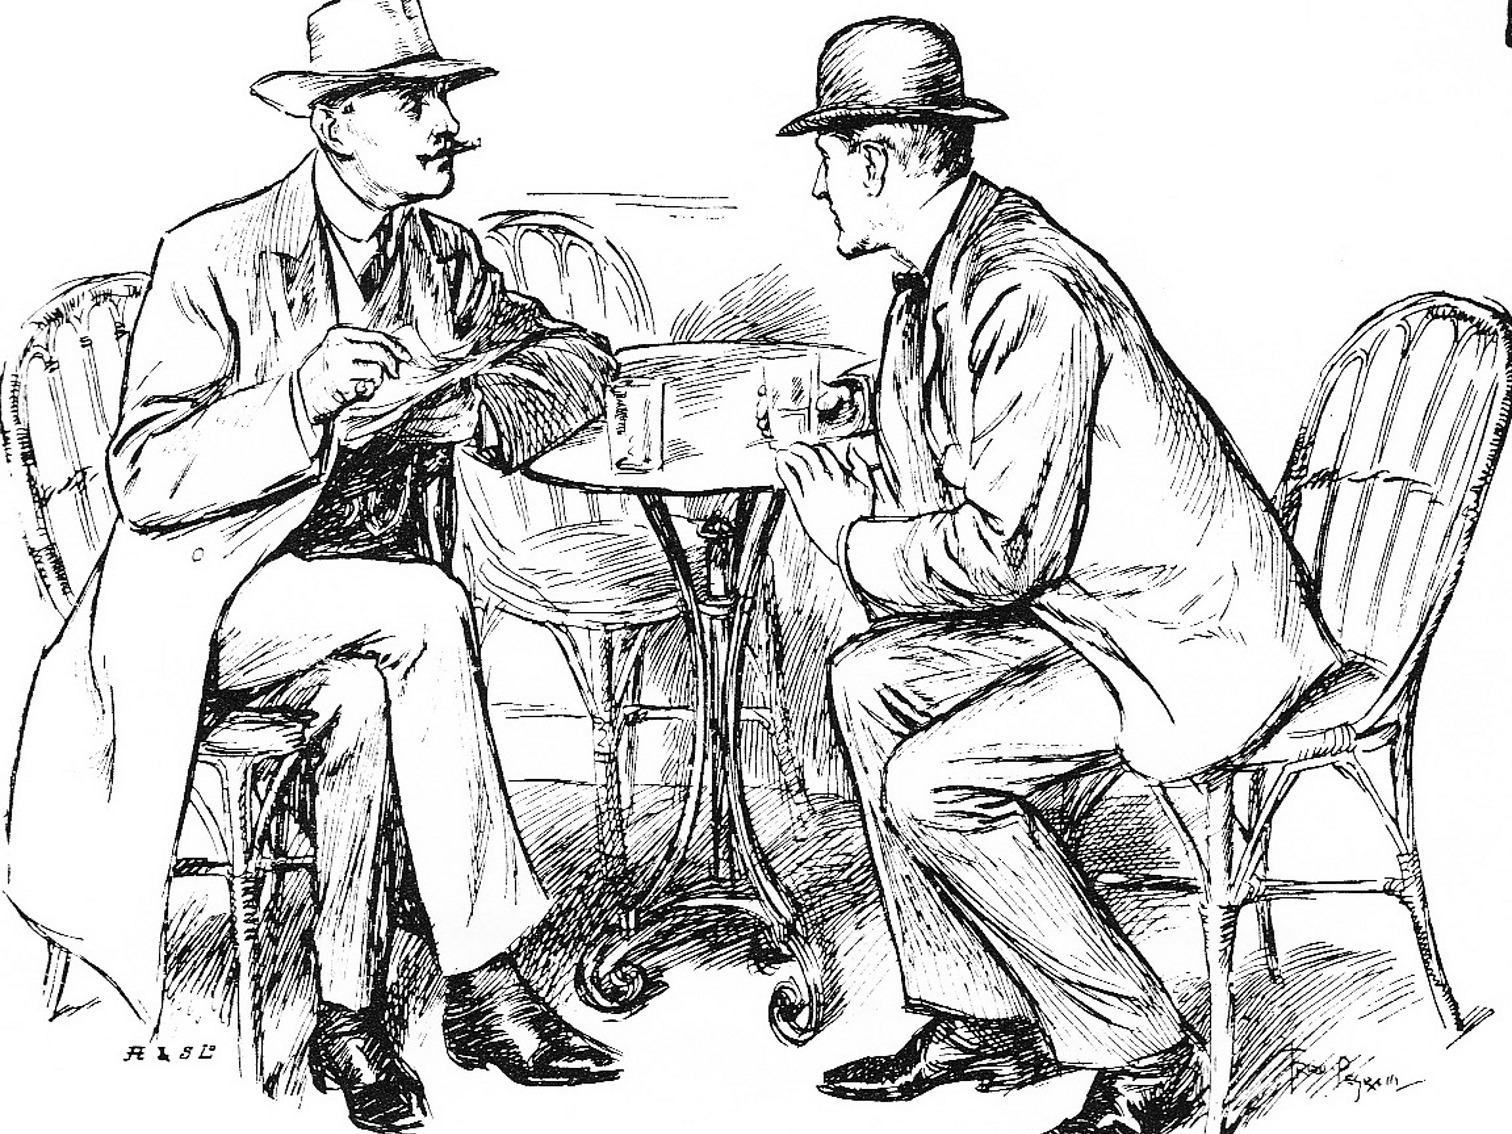
\includegraphics[scale=0.048]{1.jpg} \ flickr/lovelornpoets\\
% 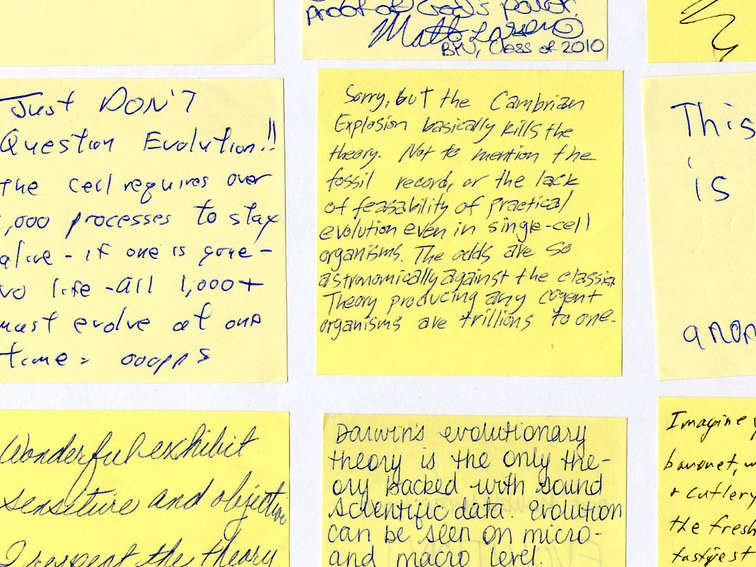
\includegraphics[scale=0.2]{2.jpg} \ flickr/apsmuseum
% }
% \end{frame}

%----------------------------------------------------------------------------------------

\end{document}